\chapter{Results}
\label{sec:results}


\section{Presentation of Collected Data}
\subsection{Overview of Interviews}
We conducted semi-structured interviews with 16 native Swedish speakers (10 M/6F, age 23-78), each lasting 1-3 minutes. Each participant was interviewed for two different scenarios, resulting in 30 different recordings. All interviews were audio-recorded in a quiet room and elicited two target emotions – anger and happiness – via open-ended prompts (e.g. “Is there anything in society that makes you upset? What? How does that make you feel?”; “Can you remember one time you felt really proud of yourself?”). The participants rated their perceived emotions on a 1-6 scale immediately after each scenario. The rated emotions covered the basic 5 emotions mentioned in this report: anger, joy, sadness, fear, and surprise. 

Table~\ref{tab:interview_table} presents the participants ID, gender, age, and self-assessed scores for their perceived emotions for respective interview scenario.
\begin{table}[H]
    \centering
    \begin{tabular}{|lrl|
    >{\columncolor[HTML]{FBE2D5}}l 
    >{\columncolor[HTML]{FBE2D5}}l 
    >{\columncolor[HTML]{FBE2D5}}l 
    >{\columncolor[HTML]{FBE2D5}}l 
    >{\columncolor[HTML]{FBE2D5}}l |
    >{\columncolor[HTML]{DAF2D0}}l 
    >{\columncolor[HTML]{DAF2D0}}l 
    >{\columncolor[HTML]{DAF2D0}}l 
    >{\columncolor[HTML]{DAF2D0}}l 
    >{\columncolor[HTML]{DAF2D0}}l |}
    \hline
    \multicolumn{3}{|c|}{Participant}                                                                                                 & \multicolumn{5}{c|}{\cellcolor[HTML]{F7C7AC}Negative}                                                                                                                                                     & \multicolumn{5}{c|}{\cellcolor[HTML]{B5E6A2}Positive}                                                                                                                                                                                                  \\ \hline
    \multicolumn{1}{|l|}{\cellcolor[HTML]{D9D9D9}ID} & \multicolumn{1}{l|}{\cellcolor[HTML]{D9D9D9}M/F} & \cellcolor[HTML]{D9D9D9}Age & \multicolumn{1}{l|}{\cellcolor[HTML]{FBE2D5}A} & \multicolumn{1}{l|}{\cellcolor[HTML]{FBE2D5}J} & \multicolumn{1}{l|}{\cellcolor[HTML]{FBE2D5}Sad} & \multicolumn{1}{l|}{\cellcolor[HTML]{FBE2D5}F} & Sur & \multicolumn{1}{c|}{\cellcolor[HTML]{DAF2D0}A} & \multicolumn{1}{c|}{\cellcolor[HTML]{DAF2D0}J} & \multicolumn{1}{c|}{\cellcolor[HTML]{DAF2D0}Sad} & \multicolumn{1}{c|}{\cellcolor[HTML]{DAF2D0}F} & \multicolumn{1}{c|}{\cellcolor[HTML]{DAF2D0}Sur} \\ \hline
    \multicolumn{1}{|l|}{1}                          & \multicolumn{1}{r|}{M}                           & 23                          & \multicolumn{1}{l|}{\cellcolor[HTML]{FBE2D5}5} & \multicolumn{1}{l|}{\cellcolor[HTML]{FBE2D5}1} & \multicolumn{1}{l|}{\cellcolor[HTML]{FBE2D5}3}   & \multicolumn{1}{l|}{\cellcolor[HTML]{FBE2D5}1} & 1   & \multicolumn{1}{l|}{\cellcolor[HTML]{DAF2D0}1} & \multicolumn{1}{l|}{\cellcolor[HTML]{DAF2D0}6} & \multicolumn{1}{l|}{\cellcolor[HTML]{DAF2D0}1}   & \multicolumn{1}{l|}{\cellcolor[HTML]{DAF2D0}1} & 4                                                \\ \hline
    \multicolumn{1}{|l|}{2}                          & \multicolumn{1}{r|}{M}                           & 26                          & \multicolumn{1}{l|}{\cellcolor[HTML]{FBE2D5}6} & \multicolumn{1}{l|}{\cellcolor[HTML]{FBE2D5}1} & \multicolumn{1}{l|}{\cellcolor[HTML]{FBE2D5}3}   & \multicolumn{1}{l|}{\cellcolor[HTML]{FBE2D5}4} & 1   & \multicolumn{1}{l|}{\cellcolor[HTML]{DAF2D0}1} & \multicolumn{1}{l|}{\cellcolor[HTML]{DAF2D0}6} & \multicolumn{1}{l|}{\cellcolor[HTML]{DAF2D0}1}   & \multicolumn{1}{l|}{\cellcolor[HTML]{DAF2D0}2} & 1                                                \\ \hline
    \multicolumn{1}{|l|}{3}                          & \multicolumn{1}{r|}{F}                           & 27                          & \multicolumn{1}{l|}{\cellcolor[HTML]{FBE2D5}4} & \multicolumn{1}{l|}{\cellcolor[HTML]{FBE2D5}1} & \multicolumn{1}{l|}{\cellcolor[HTML]{FBE2D5}6}   & \multicolumn{1}{l|}{\cellcolor[HTML]{FBE2D5}1} & 2   & \multicolumn{1}{l|}{\cellcolor[HTML]{DAF2D0}1} & \multicolumn{1}{l|}{\cellcolor[HTML]{DAF2D0}6} & \multicolumn{1}{l|}{\cellcolor[HTML]{DAF2D0}1}   & \multicolumn{1}{l|}{\cellcolor[HTML]{DAF2D0}1} & 3                                                \\ \hline
    \multicolumn{1}{|l|}{4}                          & \multicolumn{1}{r|}{M}                           & 29                          & \multicolumn{1}{l|}{\cellcolor[HTML]{FBE2D5}2} & \multicolumn{1}{l|}{\cellcolor[HTML]{FBE2D5}1} & \multicolumn{1}{l|}{\cellcolor[HTML]{FBE2D5}3}   & \multicolumn{1}{l|}{\cellcolor[HTML]{FBE2D5}2} & 1   & \multicolumn{1}{l|}{\cellcolor[HTML]{DAF2D0}1} & \multicolumn{1}{l|}{\cellcolor[HTML]{DAF2D0}4} & \multicolumn{1}{l|}{\cellcolor[HTML]{DAF2D0}2}   & \multicolumn{1}{l|}{\cellcolor[HTML]{DAF2D0}2} & 2                                                \\ \hline
    \multicolumn{1}{|l|}{5}                          & \multicolumn{1}{r|}{F}                           & 28                          & \multicolumn{1}{l|}{\cellcolor[HTML]{FBE2D5}4} & \multicolumn{1}{l|}{\cellcolor[HTML]{FBE2D5}1} & \multicolumn{1}{l|}{\cellcolor[HTML]{FBE2D5}4}   & \multicolumn{1}{l|}{\cellcolor[HTML]{FBE2D5}1} & 2   & \multicolumn{1}{l|}{\cellcolor[HTML]{DAF2D0}1} & \multicolumn{1}{l|}{\cellcolor[HTML]{DAF2D0}5} & \multicolumn{1}{l|}{\cellcolor[HTML]{DAF2D0}1}   & \multicolumn{1}{l|}{\cellcolor[HTML]{DAF2D0}1} & 5                                                \\ \hline
    \multicolumn{1}{|l|}{6}                          & \multicolumn{1}{r|}{M}                           & 25                          & \multicolumn{1}{l|}{\cellcolor[HTML]{FBE2D5}2} & \multicolumn{1}{l|}{\cellcolor[HTML]{FBE2D5}2} & \multicolumn{1}{l|}{\cellcolor[HTML]{FBE2D5}1}   & \multicolumn{1}{l|}{\cellcolor[HTML]{FBE2D5}1} & 1   & \multicolumn{1}{l|}{\cellcolor[HTML]{DAF2D0}1} & \multicolumn{1}{l|}{\cellcolor[HTML]{DAF2D0}3} & \multicolumn{1}{l|}{\cellcolor[HTML]{DAF2D0}1}   & \multicolumn{1}{l|}{\cellcolor[HTML]{DAF2D0}1} & 1                                                \\ \hline
    \multicolumn{1}{|l|}{8}                          & \multicolumn{1}{r|}{M}                           & 27                          & \multicolumn{1}{l|}{\cellcolor[HTML]{FBE2D5}3} & \multicolumn{1}{l|}{\cellcolor[HTML]{FBE2D5}1} & \multicolumn{1}{l|}{\cellcolor[HTML]{FBE2D5}2}   & \multicolumn{1}{l|}{\cellcolor[HTML]{FBE2D5}1} & 2   & \multicolumn{1}{l|}{\cellcolor[HTML]{DAF2D0}1} & \multicolumn{1}{l|}{\cellcolor[HTML]{DAF2D0}5} & \multicolumn{1}{l|}{\cellcolor[HTML]{DAF2D0}1}   & \multicolumn{1}{l|}{\cellcolor[HTML]{DAF2D0}1} & 1                                                \\ \hline
    \multicolumn{1}{|l|}{9}                          & \multicolumn{1}{r|}{F}                           & 26                          & \multicolumn{1}{l|}{\cellcolor[HTML]{FBE2D5}3} & \multicolumn{1}{l|}{\cellcolor[HTML]{FBE2D5}1} & \multicolumn{1}{l|}{\cellcolor[HTML]{FBE2D5}3}   & \multicolumn{1}{l|}{\cellcolor[HTML]{FBE2D5}1} & 1   & \multicolumn{1}{l|}{\cellcolor[HTML]{DAF2D0}1} & \multicolumn{1}{l|}{\cellcolor[HTML]{DAF2D0}5} & \multicolumn{1}{l|}{\cellcolor[HTML]{DAF2D0}1}   & \multicolumn{1}{l|}{\cellcolor[HTML]{DAF2D0}1} & 1                                                \\ \hline
    \multicolumn{1}{|l|}{10}                         & \multicolumn{1}{r|}{F}                           & 78                          & \multicolumn{1}{l|}{\cellcolor[HTML]{FBE2D5}5} & \multicolumn{1}{l|}{\cellcolor[HTML]{FBE2D5}1} & \multicolumn{1}{l|}{\cellcolor[HTML]{FBE2D5}3}   & \multicolumn{1}{l|}{\cellcolor[HTML]{FBE2D5}2} & 4   & \multicolumn{1}{l|}{\cellcolor[HTML]{DAF2D0}1} & \multicolumn{1}{l|}{\cellcolor[HTML]{DAF2D0}6} & \multicolumn{1}{l|}{\cellcolor[HTML]{DAF2D0}4}   & \multicolumn{1}{l|}{\cellcolor[HTML]{DAF2D0}1} & 1                                                \\ \hline
    \multicolumn{1}{|l|}{11}                         & \multicolumn{1}{r|}{F}                           & 27                          & \multicolumn{1}{l|}{\cellcolor[HTML]{FBE2D5}3} & \multicolumn{1}{l|}{\cellcolor[HTML]{FBE2D5}3} & \multicolumn{1}{l|}{\cellcolor[HTML]{FBE2D5}2}   & \multicolumn{1}{l|}{\cellcolor[HTML]{FBE2D5}1} & 1   & \multicolumn{1}{l|}{\cellcolor[HTML]{DAF2D0}1} & \multicolumn{1}{l|}{\cellcolor[HTML]{DAF2D0}6} & \multicolumn{1}{l|}{\cellcolor[HTML]{DAF2D0}1}   & \multicolumn{1}{l|}{\cellcolor[HTML]{DAF2D0}1} & 1                                                \\ \hline
    \multicolumn{1}{|l|}{12}                         & \multicolumn{1}{r|}{M}                           & 58                          & \multicolumn{1}{l|}{\cellcolor[HTML]{FBE2D5}1} & \multicolumn{1}{l|}{\cellcolor[HTML]{FBE2D5}3} & \multicolumn{1}{l|}{\cellcolor[HTML]{FBE2D5}1}   & \multicolumn{1}{l|}{\cellcolor[HTML]{FBE2D5}2} & 1   & \multicolumn{1}{l|}{\cellcolor[HTML]{DAF2D0}1} & \multicolumn{1}{l|}{\cellcolor[HTML]{DAF2D0}6} & \multicolumn{1}{l|}{\cellcolor[HTML]{DAF2D0}1}   & \multicolumn{1}{l|}{\cellcolor[HTML]{DAF2D0}1} & 3                                                \\ \hline
    \multicolumn{1}{|l|}{13}                         & \multicolumn{1}{r|}{F}                           & 54                          & \multicolumn{1}{l|}{\cellcolor[HTML]{FBE2D5}4} & \multicolumn{1}{l|}{\cellcolor[HTML]{FBE2D5}1} & \multicolumn{1}{l|}{\cellcolor[HTML]{FBE2D5}4}   & \multicolumn{1}{l|}{\cellcolor[HTML]{FBE2D5}3} & 1   & \multicolumn{1}{l|}{\cellcolor[HTML]{DAF2D0}1} & \multicolumn{1}{l|}{\cellcolor[HTML]{DAF2D0}6} & \multicolumn{1}{l|}{\cellcolor[HTML]{DAF2D0}1}   & \multicolumn{1}{l|}{\cellcolor[HTML]{DAF2D0}1} & 1                                                \\ \hline
    \multicolumn{1}{|l|}{14}                         & \multicolumn{1}{r|}{M}                           & 20                          & \multicolumn{1}{l|}{\cellcolor[HTML]{FBE2D5}1} & \multicolumn{1}{l|}{\cellcolor[HTML]{FBE2D5}3} & \multicolumn{1}{l|}{\cellcolor[HTML]{FBE2D5}1}   & \multicolumn{1}{l|}{\cellcolor[HTML]{FBE2D5}2} & 2   & \multicolumn{1}{l|}{\cellcolor[HTML]{DAF2D0}1} & \multicolumn{1}{l|}{\cellcolor[HTML]{DAF2D0}4} & \multicolumn{1}{l|}{\cellcolor[HTML]{DAF2D0}1}   & \multicolumn{1}{l|}{\cellcolor[HTML]{DAF2D0}1} & 3                                                \\ \hline
    \multicolumn{1}{|l|}{15}                         & \multicolumn{1}{r|}{M}                           & 30                          & \multicolumn{1}{l|}{\cellcolor[HTML]{FBE2D5}3} & \multicolumn{1}{l|}{\cellcolor[HTML]{FBE2D5}2} & \multicolumn{1}{l|}{\cellcolor[HTML]{FBE2D5}2}   & \multicolumn{1}{l|}{\cellcolor[HTML]{FBE2D5}3} & 1   & \multicolumn{1}{l|}{\cellcolor[HTML]{DAF2D0}2} & \multicolumn{1}{l|}{\cellcolor[HTML]{DAF2D0}5} & \multicolumn{1}{l|}{\cellcolor[HTML]{DAF2D0}1}   & \multicolumn{1}{l|}{\cellcolor[HTML]{DAF2D0}1} & 1                                                \\ \hline
    \multicolumn{1}{|l|}{16}                         & \multicolumn{1}{r|}{M}                           & 25                          & \multicolumn{1}{l|}{\cellcolor[HTML]{FBE2D5}4} & \multicolumn{1}{l|}{\cellcolor[HTML]{FBE2D5}1} & \multicolumn{1}{l|}{\cellcolor[HTML]{FBE2D5}2}   & \multicolumn{1}{l|}{\cellcolor[HTML]{FBE2D5}1} & 1   & \multicolumn{1}{l|}{\cellcolor[HTML]{DAF2D0}1} & \multicolumn{1}{l|}{\cellcolor[HTML]{DAF2D0}6} & \multicolumn{1}{l|}{\cellcolor[HTML]{DAF2D0}1}   & \multicolumn{1}{l|}{\cellcolor[HTML]{DAF2D0}1} & 1                                                \\ \hline
    \end{tabular}
    \caption{Participant table. A: Anger, J: Joy, Sad: Sadness, F: Fear, Sur: Surprise.}
    \label{tab:interview_table}
\end{table}

\subsection{Data Collection for RQ1: Vocal Features \& Speech}

\subsubsection{Pipeline Overview}
text ? kanske inte ha med vet ej 

\subsubsection{Structure of JSON Data Files}
\begin{center}
\begin{minipage}{0.7\textwidth} 
\begin{lstlisting}[language=json, caption={Example of stored JSON structure for vocal features vs. Hume}]
    {
    "entry_id": "id_005_neg",
    "vocal_features": {
        "mean_pitch_st": -4.12,
        "mean_pitch_hz": 118.24,
        "mean_intensity_db": 58.15,
        "mean_hnr_db": -0.5,
        "jitter_local": 0.0261,
        "shimmer_local": 0.1096,
        "formants_hz": {
            "F1": 1118.56,
            "F2": 2623.03,
            "F3": 3611.26
        }
    },
    "praat_scores": {
        "anger": 0.208,
        "joy": 0.205,
        "fear": 0.199,
        "sadness": 0.19,
        "surprise": 0.198
    },
    "praat_label": "anger",
    "hume_probs": {
        "anger": 0.21,
        "fear": 0.16,
        "joy": 0.15,
        "sadness": 0.34,
        "surprise": 0.14
    },
    "hume_label": "sadness"
}
\end{lstlisting}
\end{minipage}
\end{center} 
\subsubsection{Segment-Level Data}
text

\subsection{Data Collection for RQ2 and RQ3: Text, Speech and Self-Assessment}
\label{sec:datacoll_rq2_rq3}


The data collection for RQ2 and RQ3 is based on the same audio recordings as for RQ1. 
Each recording was transcribed and analyzed with NLP Cloud (text-based), to extract emotion probabilities from the transcription. The same audio was analyzed using Hume AI for speech-based emotion detection, resulting in paired emotion probability scores alongside self-reported emotion ratings. All scores were normalized for comparison.

The data was structured in JSON format as shown in Figure~\ref{tab:json_rq2_rq3}, each audio object consists of five emotion labels from each data type (Hume, NLP, Self). 

\begin{center}
    \begin{minipage}{0.7\textwidth} 
    \begin{lstlisting}[language=json, caption={Example of stored JSON structure for Hume, NLP, Self-labeling.}]
        {
            "id_013_neg": {
                "audio_file": "audio_use/negative/13-neg.m4a",
                "nlp_emotions": {
                    "anger": 0.44,
                    "joy": 0.0,
                    "sadness": 0.31,
                    "fear": 0.21,
                    "surprise": 0.05
                },
                "hume_emotions": {
                    "anger": 0.32,
                    "fear": 0.13,
                    "joy": 0.22,
                    "sadness": 0.19,
                    "surprise": 0.13
                },
                "self_assessed": {
                    "anger": 0.31,
                    "joy": 0.08,
                    "sadness": 0.31,
                    "fear": 0.23,
                    "surprise": 0.08
                }
            }
    }
    \end{lstlisting}
    \label{tab:json_rq2_rq3}
\end{minipage}
\end{center} 

Table~\ref{tab:summery_rq2_rq3} summarize the average emotion scores and standard deviations for both speech-based (Hume AI) and text-based (NLP Cloud) 
models across all clips in the dataset. 

\begin{table}[H]
    \begin{tabular}{c|l|l|l|l|l|l}
    \textbf{Emotion}  & \multicolumn{1}{c|}{\textbf{Self Mean}} & \multicolumn{1}{c|}{\textbf{Hume Mean}} & \multicolumn{1}{c|}{\textbf{NLP Mean}} & \multicolumn{1}{c|}{\textbf{Self Std}} & \multicolumn{1}{c|}{\textbf{Hume Std}} & \multicolumn{1}{c}{\textbf{NLP Std}} \\ \hline
    \textbf{Anger}    & 0,21                                               & 0,26                                    & 0,2                                    & 0,124                                           & 0,072                                  & 0,223                                \\
    \textbf{Joy}      & 0,312                                              & 0,302                                   & 0,396                                  & 0,2                                             & 0,117                                  & 0,351                                \\
    \textbf{Sadness}  & 0,19                                               & 0,167                                   & 0,181                                  & 0,105                                           & 0,065                                  & 0,138                                \\
    \textbf{Fear}     & 0,136                                              & 0,15                                    & 0,093                                  & 0,061                                           & 0,045                                  & 0,092                                \\
    \textbf{Surprise} & 0,149                                              & 0,118                                   & 0,129                                  & 0,082                                           & 0,022                                  & 0,089                               
    \end{tabular}
    \caption{Mean and standard deviation for Hume, NLP, Self-labeling for full dataset.}
    \label{tab:summery_rq2_rq3}
\end{table}

The interviews were conducted with either a positive or negative orientation. Each recording was analyzed individually, and
the data structure distinguishes between negative and positive audio files. The corresponding emotion scores from Hume AI and 
NLP Cloud are presented in Table~\ref{tab:summery_hume_nlp_neg} for negatively oriented interviews, and in Table~\ref{tab:summery_hume_nlp_pos}
for positively oriented interviews. Each table displays the mean and the standard deviation for the respective AI model's emotion probability. 

\begin{table}[H]
    \centering
    \begin{tabular}{lllll}
    \multicolumn{5}{c}{\cellcolor[HTML]{BFBFBF}Negative}                                                                                                                                                \\ \hline
    \multicolumn{1}{|l|}{\textbf{Emotion}}  & \multicolumn{1}{c|}{\textbf{Hume M}} & \multicolumn{1}{c|}{\textbf{NLP M}} & \multicolumn{1}{c|}{\textbf{Hume Sd}} & \multicolumn{1}{c|}{\textbf{NLP Sd}} \\ \hline
    \multicolumn{1}{|l|}{\textbf{Anger}}    & 0,29                                 & 0,363                               & 0,072                                 & 0,183                                \\ \cline{1-1}
    \multicolumn{1}{|l|}{\textbf{Joy}}      & 0,276                                & 0,121                               & 0,098                                 & 0,205                                \\ \cline{1-1}
    \multicolumn{1}{|l|}{\textbf{Sadness}}  & 0,171                                & 0,282                               & 0,066                                 & 0,104                                \\ \cline{1-1}
    \multicolumn{1}{|l|}{\textbf{Fear}}     & 0,152                                & 0,141                               & 0,038                                 & 0,087                                \\ \cline{1-1}
    \multicolumn{1}{|l|}{\textbf{Surprise}} & 0,112                                & 0,092                               & 0,021                                 & 0,064                                \\ \cline{1-1}
    \end{tabular}
    \caption{Mean and standard deviation for Hume and NLP for negative interviews.}
    \label{tab:summery_hume_nlp_neg}
\end{table}


\begin{table}[H]
    \centering
    \begin{tabular}{lllll}
    \multicolumn{5}{c}{\cellcolor[HTML]{BFBFBF}Positive}                                                                                                                                           \\
    \multicolumn{1}{l|}{\textbf{Emotion}}  & \multicolumn{1}{c}{\textbf{Hume M}} & \multicolumn{1}{c}{\textbf{NLP M}} & \multicolumn{1}{c}{\textbf{Hume Sd}} & \multicolumn{1}{c}{\textbf{NLP Sd}} \\ \hline
    \multicolumn{1}{l|}{\textbf{Anger}}    & 0,228                               & 0,015                              & 0,06                                 & 0,057                               \\
    \multicolumn{1}{l|}{\textbf{Joy}}      & 0,334                               & 0,708                              & 0,132                                & 0,168                               \\
    \multicolumn{1}{l|}{\textbf{Sadness}}  & 0,164                               & 0,067                              & 0,065                                & 0,062                               \\
    \multicolumn{1}{l|}{\textbf{Fear}}     & 0,148                               & 0,04                               & 0,053                                & 0,068                               \\
    \multicolumn{1}{l|}{\textbf{Surprise}} & 0,126                               & 0,171                              & 0,022                                & 0,097                              
    \end{tabular}
    \caption{Mean and standard deviation for Hume and NLP for positive interviews.}
    \label{tab:summery_hume_nlp_pos}
\end{table}

\section{Data Analysis for RQ1: Vocal Features \& Speech Emotion Recognition}

\subsection{Correlation Between Vocal Features and AI Emotion Scores (Hume AI)}

\begin{figure}[H]
    \centering
    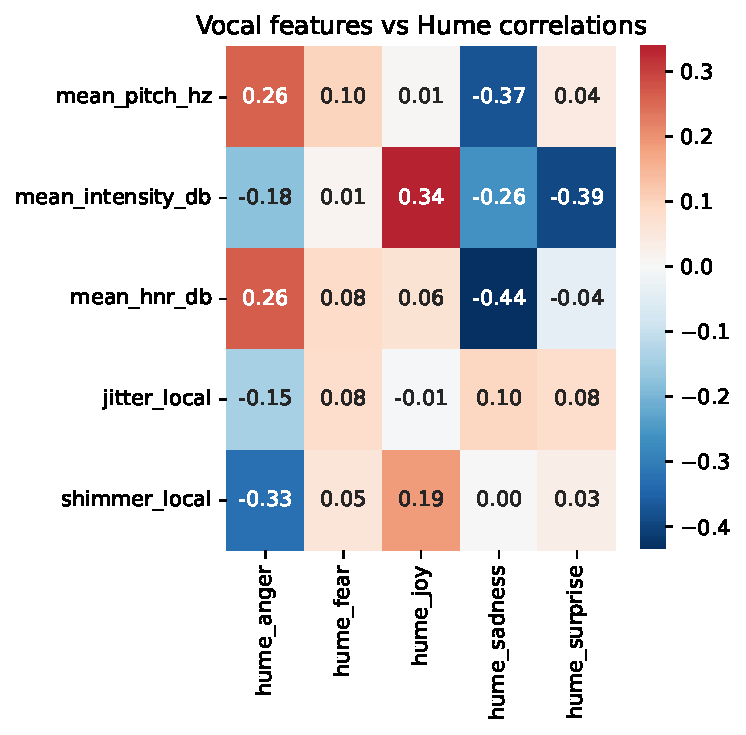
\includegraphics[width=0.5\textwidth]{png/results/rq1/vocal_features_vs_hume_correlations.pdf}
    \caption{Heatmap of correlation between vocal markers and Hume labels.}
    \label{fig:heatmap-voc-hume}
\end{figure}

Figure~\ref{fig:heatmap-voc-hume} demonstrates a heatmap of the Pearson correlation coefficients between selected vocal features and Hume AI emotion labels across all clips in the dataset. The results show generally weak correlations, with most values in the range of -0.4 and 0.3. 

\medskip
Key findings: 
\begin{itemize}
    \item Mean pitch (Hz) shows a moderate correlation with sadness (r = -0.37). 
    \item Mean Intensity (dB) has a moderate positive correlation with joy (r = 0.34) and a moderate negative correlation with surprise(r = -0.39). These results align with the referred research indicating that vocal intensity tends to increase with positive arousal states \autocite{Ekberg2023}. 
    \item Mean HNR has a moderate negative correlation with sadness (r = -0.44), but shows weak correlations across all other emotions.
    \item Shimmer shows a moderate negative correlation with anger (-0.33).
    \item Jitter and shimmer showed overall weak correlations, which may reflect that these features are subtle in spontaneous speech contexts compared to controlled or acted settings.  
\end{itemize}
Overall, the correlations with Hume suggest minor tendencies that reflect known vocal-emotion relationships, especially regarding pitch and intensity. The low degree of these correlations indicates that selected acoustic features alone did not strongly predict AI-detected emotions. 

\subsection{Correlation with Praat-Based Emotion Scores}

\begin{figure}[H]
    \centering
    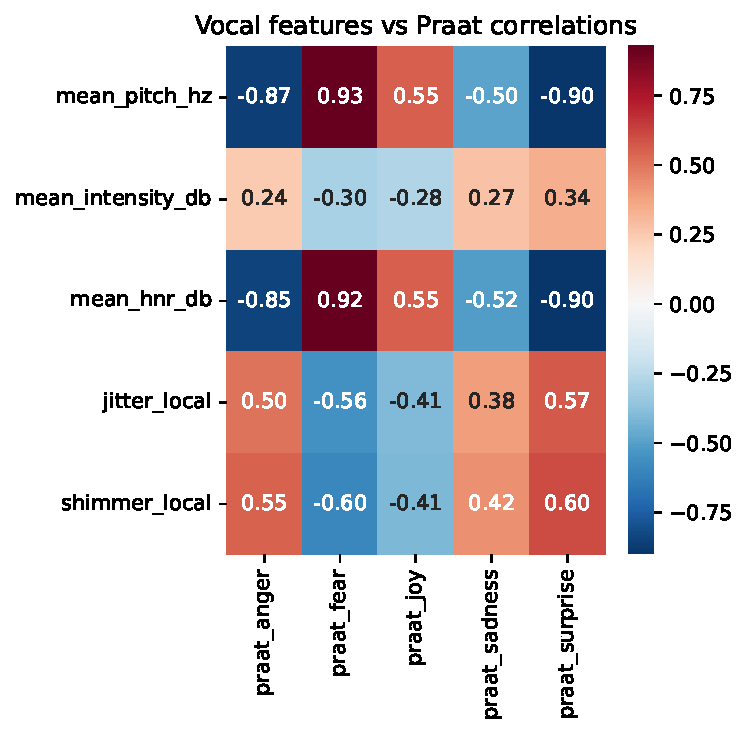
\includegraphics[width=0.5\textwidth]{png/results/rq1/vocal_features_vs_praat_correlations.pdf}
    \caption{Heatmap of correlation between vocal markers and custom emotion categorization.}
    \label{fig:heatmap-voc-praat}
\end{figure}
Figure~\ref{fig:heatmap-voc-praat} illustrates correlation between vocal features and the emotion scores obtained from the custom Praat-based categorization function. In contrast to the results for Hume, these correlations are notably higher. However, it shows patterns that are inconsistent with theoretical expectations. 
\medskip
Key findings: 
\begin{itemize}
    \item Mean pitch (Hz) shows very strong correlations (r = -0.87) with anger and fear (r = 0.93), which suggests that pitch strongly impacted the outcomes of the categorization. 
    \item Mean HNR (dB) revealed similar strong correlations as pitch, with high values for anger (r = -0.85) and fear (r = 0.92). 
    \item Jitter and shimmer display moderate to strong correlations as well, with varying directions for different emotions. 
\end{itemize}
The results suggest that the Praat-based function weighted some vocal features very heavily, especially pitch and HNR, resulting in inflated correlations that may be misleading. The absence of varying differences across the emotions suggest that the rule-based approach did not capture some expressions in spontaneous, interviewed, speech. 

\subsection{Limitations of the Custom Vocal Emotion Categorization Method}
To evaluate the performance of our custom emotion categorization function, which was developed based on vocal markers reported in the Swedish study \autocite{Ekberg2023}, we compared the emotion labels to the labels generated by Hume AI’s speech-based emotion recognition model. This comparison included both individual clip level and across the full dataset. 

However, the results revealed significant limitations in our approach. Regardless of the vocal input from our dataset, the categorization function consistently rendered near homogeneous emotion scores across all five emotions. This indicates that the function failed to capture emotional distinctions within spontaneous, conversational speech during interviews, regardless of theoretical relevance. 

Figure~\ref{fig:scatter_hume_praat} illustrates this issue across the full dataset, where the average scores assigned by our Praat-based categorization remain clustered around 0.2 across all emotions. Opposed to Hume that had greater variation through its labeling and reflects a more dynamic emotional detection.

\begin{figure}[H]
    \centering
    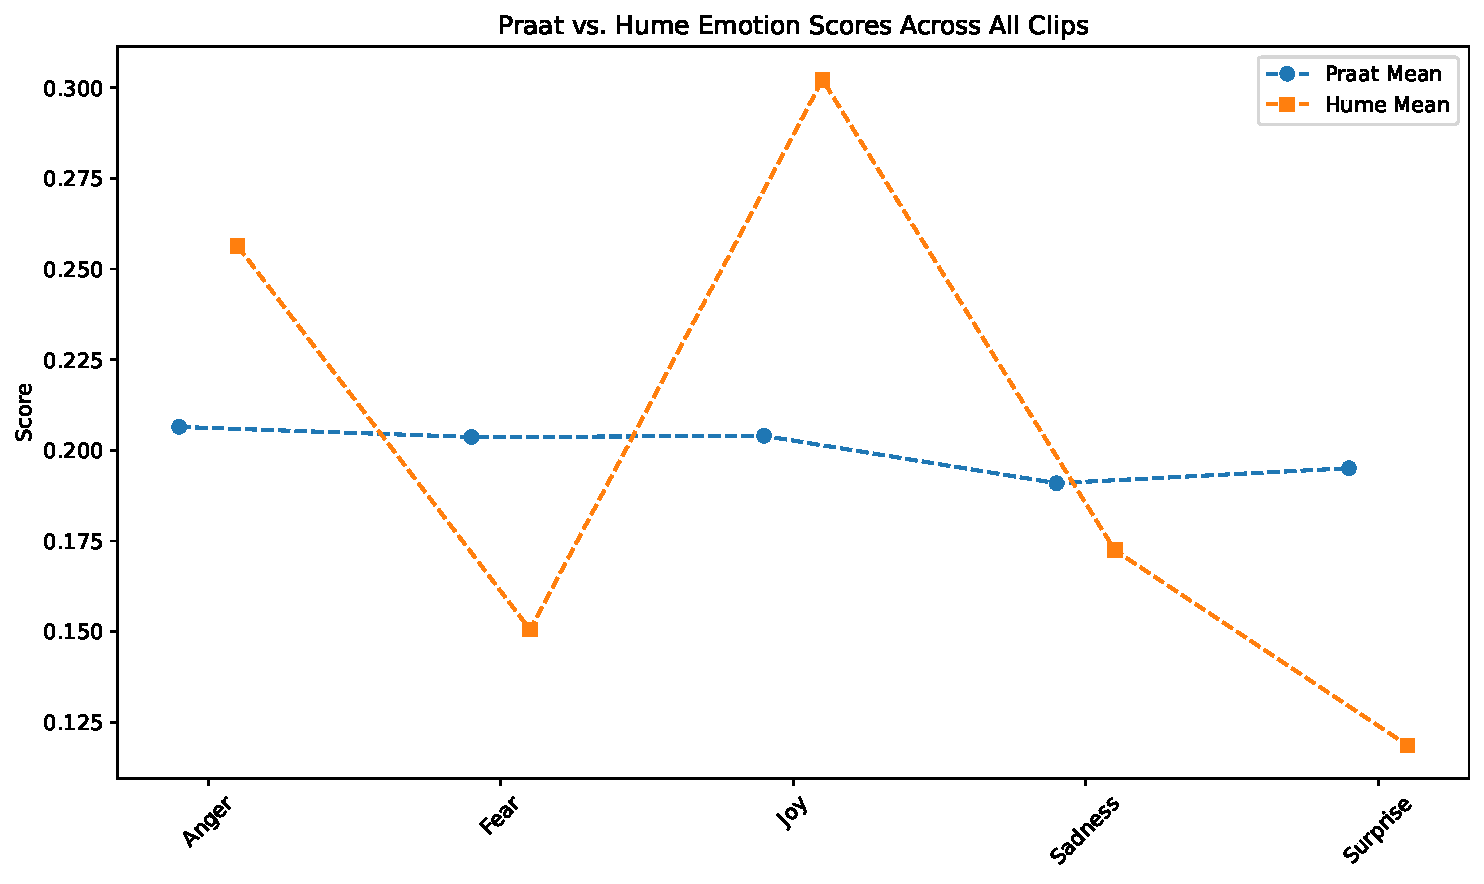
\includegraphics[width=0.7\textwidth]{png/results/rq1/praat_hume_all_clips_scatter.pdf}
    \caption{Average Score of vocal features-categorization and Hume labeling across all clips.}
    \label{fig:scatter_hume_praat}
\end{figure}

This is presented similarly in Figure~\ref{fig:praat_hume_008}, which presents a comparison for a single negative directed interview \texttt{id\_008\_neg}. In the same way as in Figure~\ref{fig:scatter_hume_praat}, the Praat-based scores are distributed very evenly across all emotions, while Hume assigns a higher probability to anger and lower for surprise,
with joy, sadness, and fear clustered more closely. Despite the fact that the score diversity between the Hume-labeled emotions are relatively moderate - approximately 0.10 between anger and sadness/joy, and around 0.15 between surprise and sadness/joy - the probabilities are still more diverse and provide a more interpretable output. The variability could be considered more reflective of potential emotional nuances in the interview. 

These findings demonstrate that our vocal feature-based categorization lacked sensitivity and adaptability when applied to our interview-based Swedish speech data. As a result, subsequent analyses focused on direct comparisons between raw vocal features and AI-predicted emotions, instead of relying on this flawed categorization method. 
\begin{figure}[H]
    \centering
    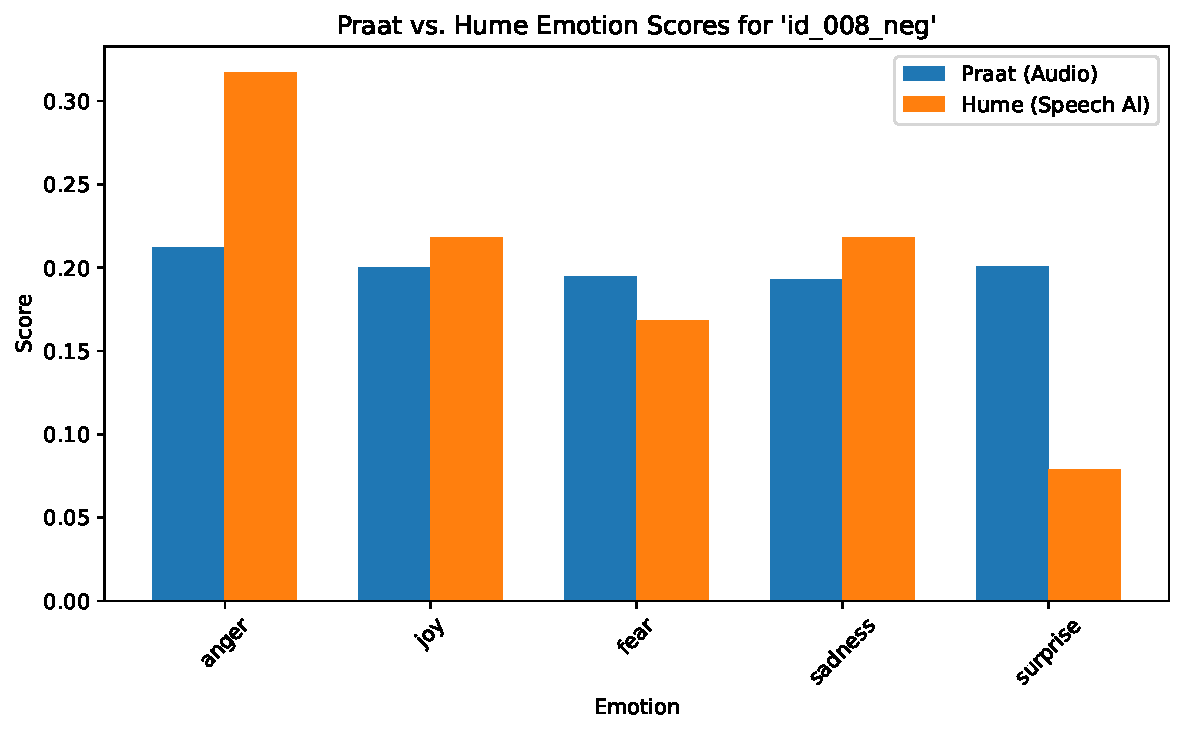
\includegraphics[width=0.7\textwidth]{png/results/rq1/id_008_neg_praat_hume_comparison.pdf}
    \caption{Vocal feature-categorization vs. Hume for single clip.}
    \label{fig:praat_hume_008}
\end{figure}

\subsection{ANOVA Summery of Vocal Features Across Emotions}
An ANOVA was implemented to further examine whether essential vocal features varied across AI-labeled emotions. This was conducted on pitch, intensity, HNR, jitter, and shimmer. The results are summarised in Table~\ref{tab:anova-rq1} and showed that none of the features showed statistically significant differences between the five Hume emotion categories (all p-values > 0.23). To confirm these findings, Tukey HSD tests were conducted and resulted in no pairwise comparisons between emotion labels with significant difference. 

\begin{table}[H]
    \centering
    \begin{tabular}{l|r|rrr}
    \multicolumn{1}{c|}{\textbf{Feature}} & \multicolumn{1}{c|}{\textbf{ANOVA p-value}} & \multicolumn{1}{c}{\textbf{Significant Differences}} &  &  \\ \cline{1-3}
   
    mean\_pitch\_hz                      & 0,4435                                     & No                                                   &  &  \\
    mean\_intensity\_db                  & 0,5793                                     & No                                                   &  &  \\
    mean\_hnr\_db                        & 0,2327                                     & No                                                   &  &  \\
    jitter\_local                        & 0,7797                                     & No                                                   &  &  \\
    shimmer\_local                       & 0,385                                      & No                                                   &  & 
    \end{tabular}
    \caption{ANOVA table for vocal features variance across emotions}
    \label{tab:anova-rq1}
\end{table}
These results imply that within our dataset of spontaneous speech during interviews, the average values of the acoustic features did not systematically vary according to AI-labeled emotions. This could indicate that emotional expression in conversations during interview circumstances is either: 
\begin{itemize}
    \item More subtle than in controlled studies.
    \item Features like pitch and intensity fluctuate instead of differing consistently at the audio clip level. 
    \item A deficient set of vocal features were extracted for these analyses. 
\end{itemize}
The lack of variance in these results does not align with findings in controlled settings \autocite{Ekberg2023}, where clear differences in vocal features were found between different emotional states. 

\subsection{Correlation Between Vocal Features and Hume AI Emotion Scores}
Considering the limitations that had been identified in our vocal feature-based emotion categorization function, subsequent analyses shifted focus towards examining direct correlation between raw acoustic features and AI-predicted emotions. Instead of applying predefined vocal emotion mappings to rely on, essential vocal markers have been investigated to obtain an understanding of how these correlate with Hume AI’s emotion scores across our dataset. 

\subsubsection{Composite Correlation Overview}
Figure~\ref{fig:composite} illustrates a composite correlation analysis, including Pearson correlation coefficients (r) between two acoustic features - pitch and intensity - and the given emotion categories that are filtered from Hume AI. Even if the correlations are generally moderate, certain patterns appear which aligns with previous findings in vocal emotion research. 
\begin{figure}[H]
    \centering 
    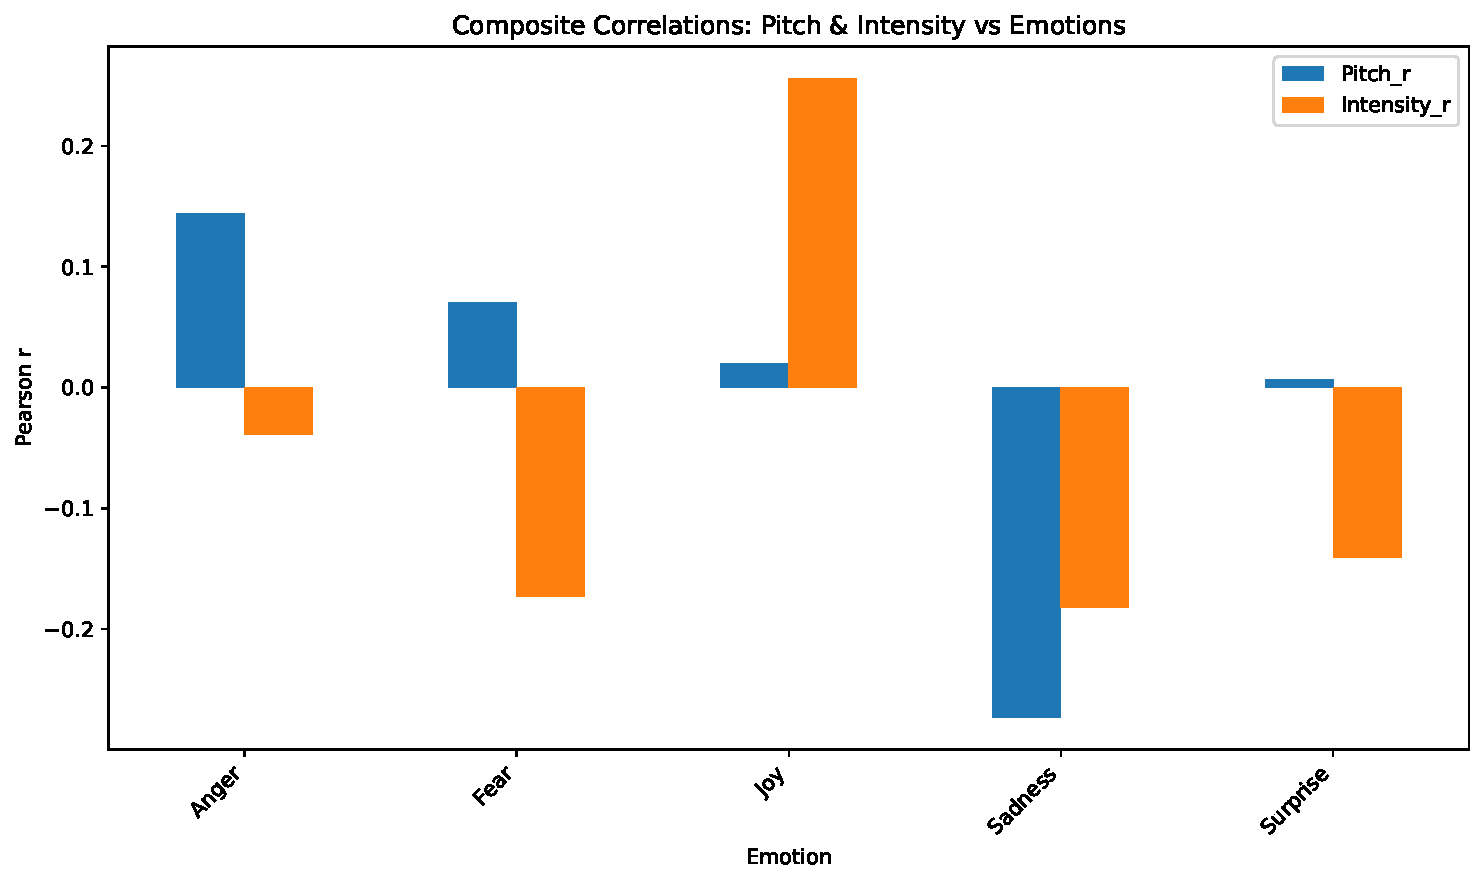
\includegraphics[width=0.6\textwidth]{png/results/rq1/composite_correlations.pdf}
    \caption{Composite correlation analysis}
    \label{fig:composite}
\end{figure}

Particularly intensity shows a positive correlation with joy, and suggests that higher vocal intensity tends to co-occur with AI detected happiness. In contrast, intensity shows a negative correlation with emotions such as sadness and fear, which is aligned with the expectations that these emotions are generally expressed with lower vocal energy. 

For pitch, a minor positive correlation is found in correlation with anger and fear, also reflecting expectations reported in prior research, where higher pitch is associated with heightened arousal states, for example anger. A negative correlation between pitch and sadness is shown, also supporting the prior findings where sadness is linked to lower pitch. 

However, the correlation strength is weak across all emotions, without values that indicate a strong linear association. This indicates, as our previous results, that single acoustic features like pitch and intensity alone are insufficient markers of emotional states when detected by speech emotion recognition systems, in the context of conversational, but interviewed, speech. 

\subsubsection{Supporting observations from individual clips}

For a more concrete illustration of the prior tendencies stated, two interview recordings were analyzed in detail. The purpose was to examine whether emotional shifts become more apparent when evaluating shorter time segments within individual speakers, compared to the weaker correlations observed at the dataset level.

In Figure~\ref{fig:pitch-4-pos} and \ref{fig:intensity-4-pos}, data is demonstrated from a positively directed interview \texttt{id\_004\_pos}, female, which shows that increases in pitch and intensity considerably often correlate with higher joy probabilities by Hume AI. While the correlation is not consistent throughout the recording, these moment-to-moment variations reflect the general expectation that higher vocal energy is associated with positive emotional expression. 

\begin{figure}[H]
    \centering
    \begin{subfigure}[b]{0.47\textwidth}
        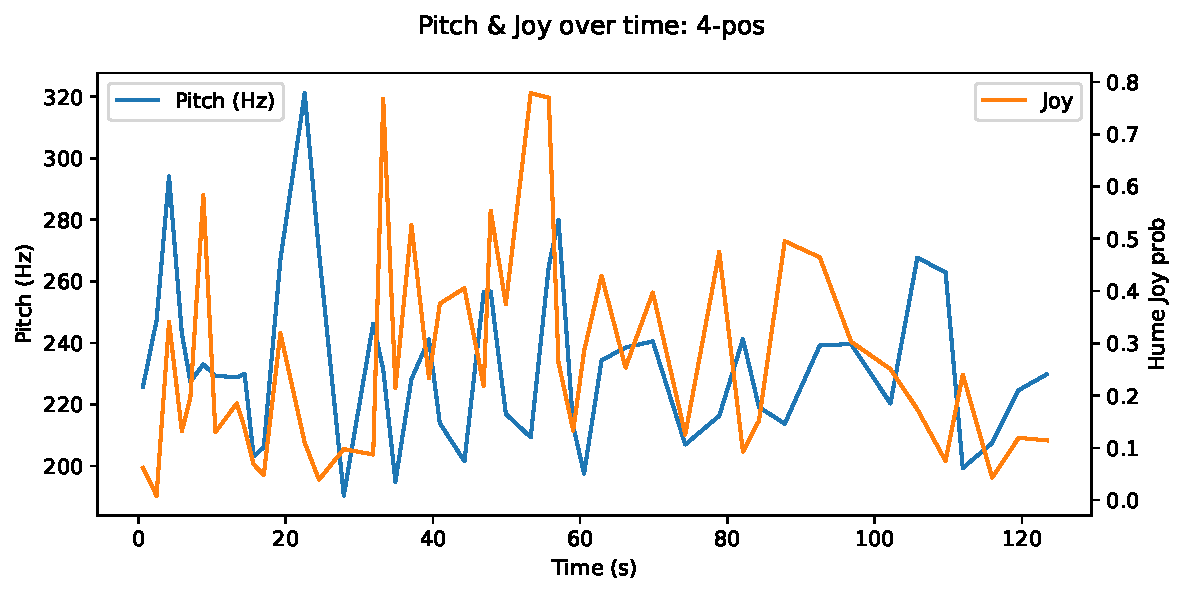
\includegraphics[width=\linewidth]{png/results/rq1/pitch_joy_4-pos.pdf}
        \caption{Pitch(Hz) and Hume label joy over time. Clip 4-pos}
        \label{fig:pitch-4-pos}
    \end{subfigure}
    \hspace{0.04\textwidth}
    \begin{subfigure}[b]{0.47\textwidth}
        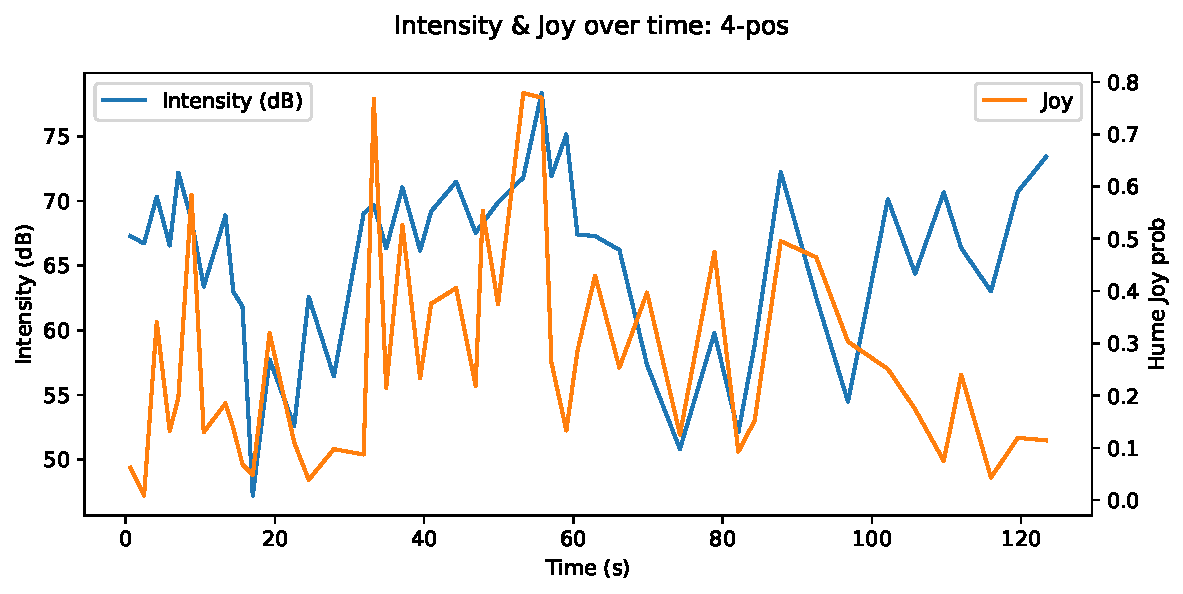
\includegraphics[width=\linewidth]{png/results/rq1/intensity_joy_4-pos.pdf}
        \caption{Intensity(dB) and Hume label joy over time. Clip 4-pos}
        \label{fig:intensity-4-pos}
    \end{subfigure}
\end{figure}

Similarly, Figure~\ref{fig:pitch-15-neg} and \ref{fig:intensity-15-neg} and \ref{fig:z-score-15} present data from a negatively directed interview \texttt{id\_015\_neg}, male. Here, clear peaks in pitch and intensity correspond with increased anger probabilities. These results are partly aligned with prior research on vocal markers of high-arousal negative emotions, such as raised pitch and loudness during expressed anger. 

\begin{figure}[H]
    \centering
    \begin{subfigure}[b]{0.47\textwidth}
        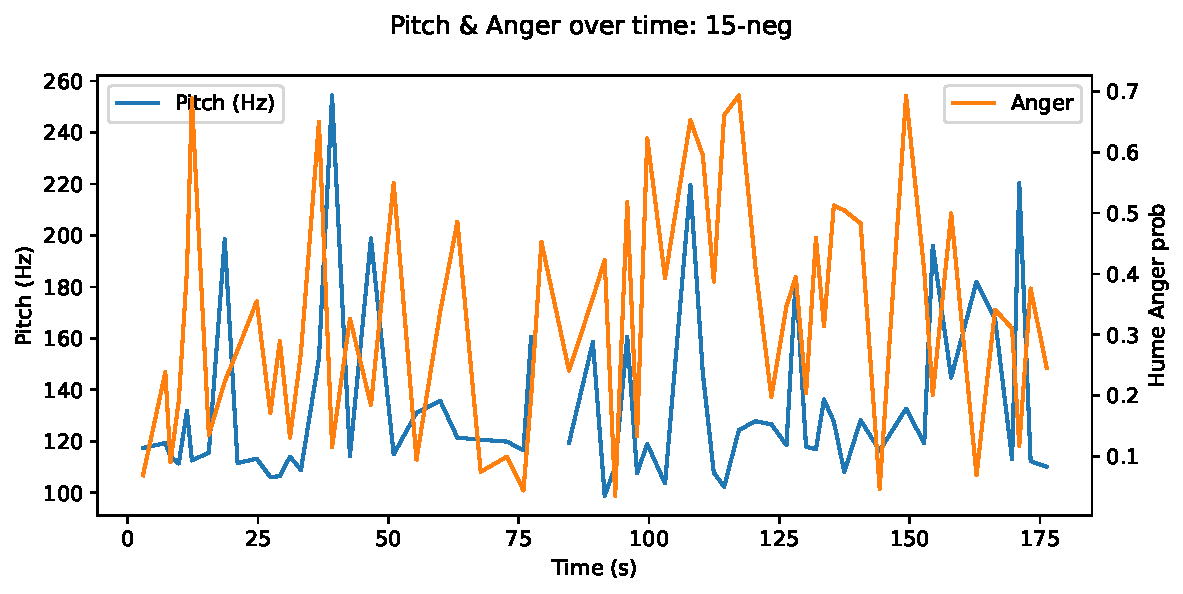
\includegraphics[width=\linewidth]{png/results/rq1/pitch_anger_15-neg.pdf}
        \caption{Pitch(Hz) and Hume label joy over time. Clip 15-neg}
        \label{fig:pitch-15-neg}
    \end{subfigure}
    \hspace{0.04\textwidth}
    \begin{subfigure}[b]{0.47\textwidth}
        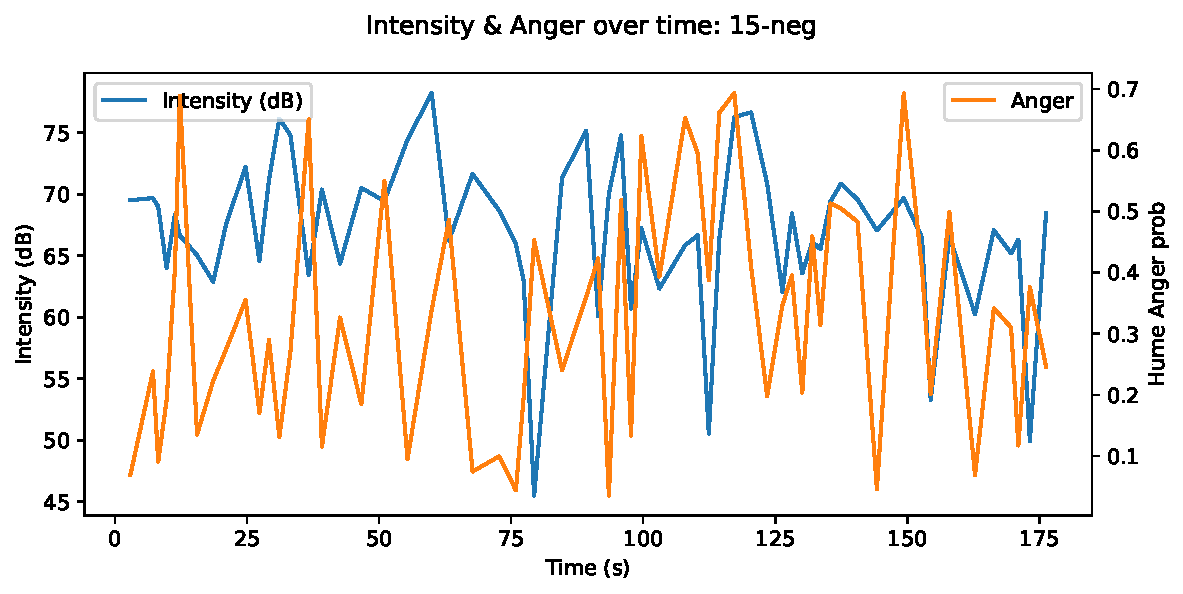
\includegraphics[width=\linewidth]{png/results/rq1/intensity_anger_15-neg.pdf}
        \caption{Intensity(dB) and Hume label joy over time. Clip 15-neg}
        \label{fig:intensity-15-neg}
    \end{subfigure}
\end{figure}

Additionally, Figure C illustrates z-score fluctuations of key vocal features for clip 13-neg. For this interview, several segments exceed +-1 standard deviation from the baseline, especially for pitch, intensity, and shimmer. These flagged moments align frequently with the emotion probabilities of Hume, which strengthens the link between vocal patterns and perceived emotional intensity. 

The z-score fluctuation diagram Figure \ref{fig:z-score-15} illustrates the segments further where vocal features significantly deviate from baseline levels, in patterns aligned with associated high-arousal negative emotions such as raised pitch and loudness. 

\begin{figure}[H]
    \centering 
    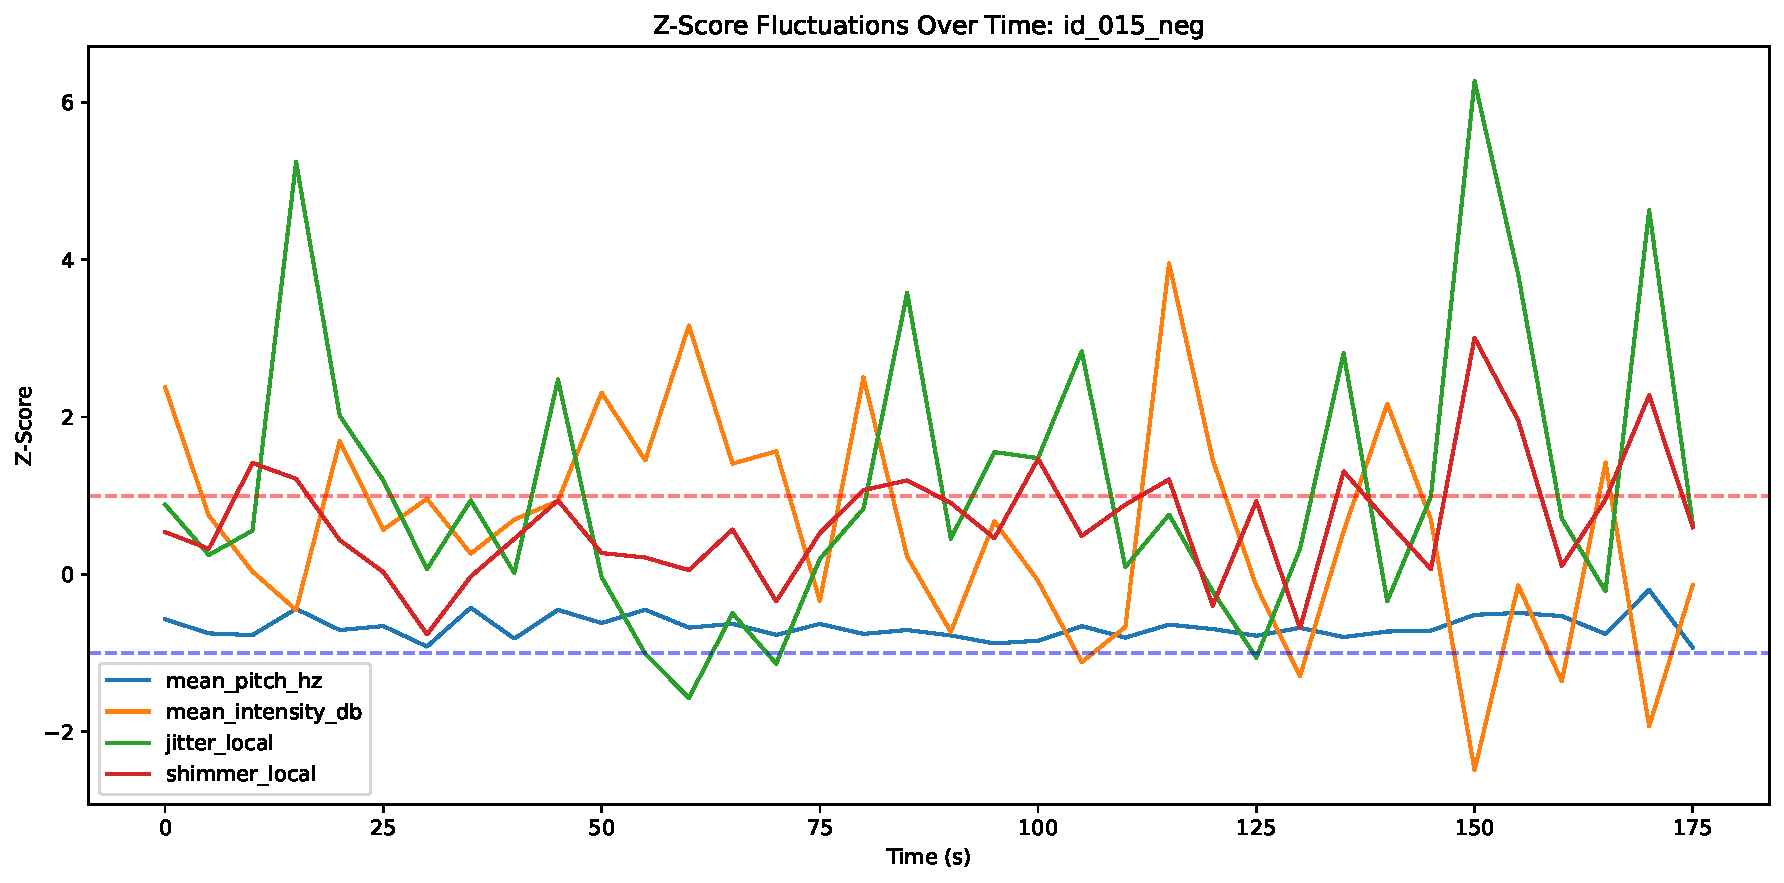
\includegraphics[width=0.7\textwidth]{png/results/rq1/zscore_fluctuations_id_015_neg.pdf}
    \caption{Z-score}
    \label{fig:z-score-15}
\end{figure}

\subsubsection{Summery}
This supports the idea that analyzing how vocal features change over time  can provide more meaningful insights into emotional expression in conversational, partly spontaneous speech during interviews compared to only using overall clip-level statistics.


%%%%%%%%%%%% RQ2 %%%%%%%%%%%%%%%%%%
\section{Data Analysis for RQ2: Text and Speech Based Emotion Recognition}
Text 
\subsection{Overall Comparison of AI Systems}
To compare the overall performance and certain tendencies of the two AI-based emotion recognition systems (Hume AI and NLP Cloud),
both descriptive statistics and visual analyses were conducted to interpret the results through calculating the average differences.

As presented in Table~\ref{tab:summery_rq2_rq3}, Table~\ref{tab:summery_hume_nlp_neg}, and Table~\ref{tab:summery_hume_nlp_pos} (\ref{sec:datacoll_rq2_rq3}),
the mean emotion scores and standard deviations differ between the two models across the full dataset,
including patterns within positive and negative interviews. 

Figure~\ref{fig:comp_bar_full_rq2} illustrates the average difference in emotion scores between Hume AI and NLP Cloud across the full dataset. Positive values indicate that Hume AI assigned 
higher scores for the respective emotion, while negative values implies higher scores from NLP Cloud. The most evident difference was shown for Joy, where 
NLP Cloud consistently provided higher scores compared to Hume AI. In contrast, Fear and Anger had a higher tendency to be detected by Hume AI. 
Differences for Sadness and Surprise were insignificant, which suggests general agreement between the systems for these emotions. 

shows that Hume AI generally compose higher scores for Fear and Sadness, while NLP Cloud assigned higher values for 
Joy and Anger to some extent. Still, the differences were relatively small across the majority of emotions, 
except for Fear, where Hume showed a prominent higher pattern. 

\begin{figure}[!h]
    \centering
    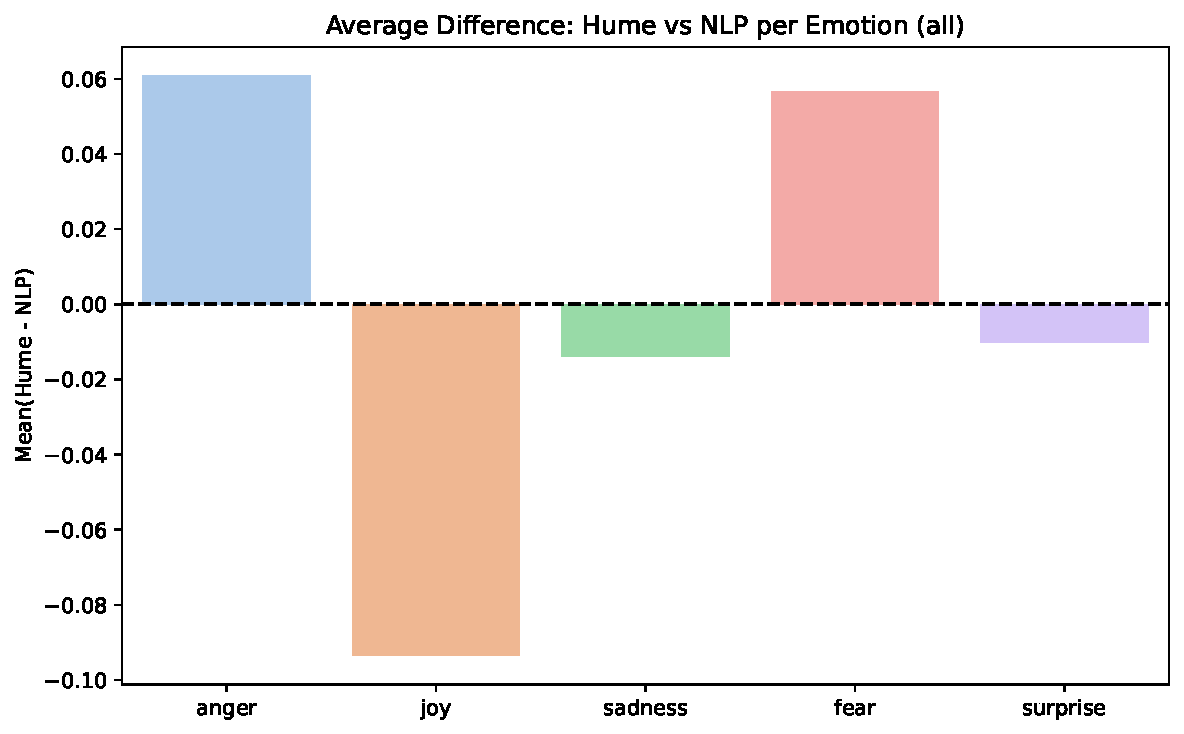
\includegraphics[width=0.7\textwidth]{png/results/rq2/hume_nlp_difference_all.pdf}
    \caption{Average difference in emotion scores between Hume AI and NLP Cloud}
    \label{fig:comp_bar_full_rq2}
\end{figure}

%%% TA BORT???%%% 
\begin{figure}
\centering
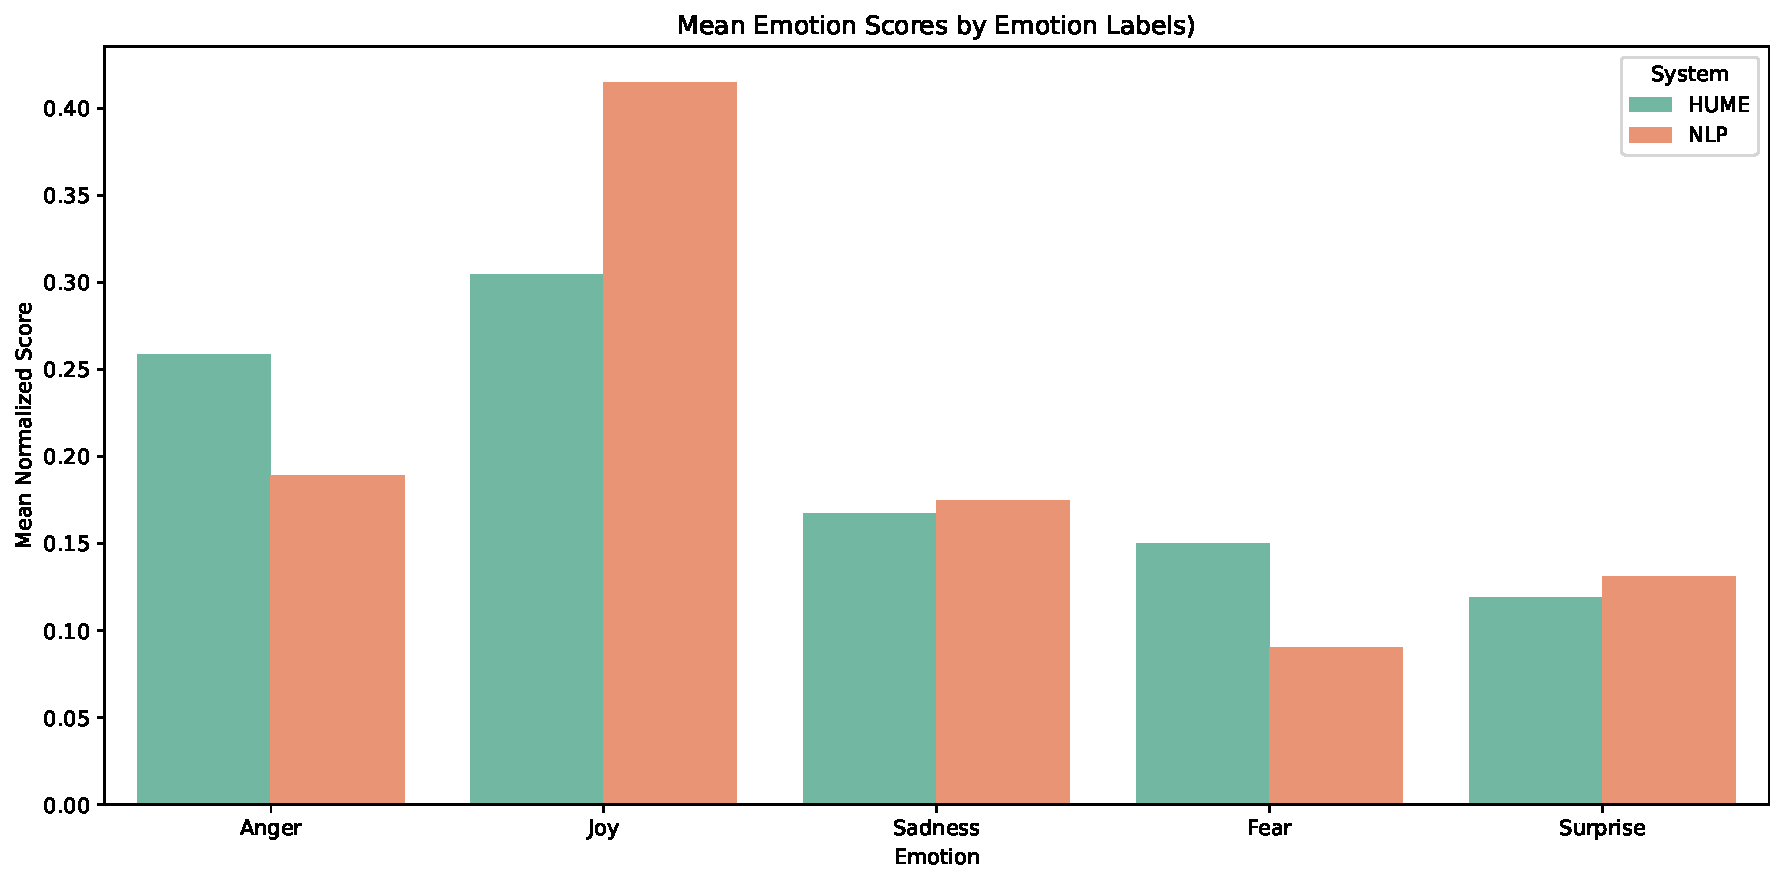
\includegraphics[width=0.7\textwidth]{png/results/rq2/sentiment_comparison_bar.pdf}
\caption{Comparison bar between Hume and NLP emotion scores for full dataset.}
\label{fig:sentiment_bar_full_rq2}
\end{figure}

\newpage
\subsection{Statistical Analysis}
\subsubsection{Correlation Analysis}

To evaluate how text-based (NLP Cloud) and speech-based (Hume AI) emotion recognition aligns, Pearson correlation coefficients (r) were calculated for each emotion across all interview recordings. 
Table~\ref{tab:pearson-pval-rq2} presents the correlation values as well as corresponding p-values to examine the statistical significance. 

\begin{table}[!h]
    \centering
    \begin{tabular}{c|ll}
    \rowcolor[HTML]{C0C0C0} 
    \textbf{Emotion}  & \multicolumn{1}{c}{\cellcolor[HTML]{C0C0C0}\textbf{Pearson r}} & \multicolumn{1}{c}{\cellcolor[HTML]{C0C0C0}\textbf{p-value}} \\ \hline
    \textbf{Anger}    & 0,468                                                          & 0,0069                                                       \\
    \textbf{Joy}      & 0,521                                                          & 0,0022                                                       \\
    \textbf{Sadness}  & 0,166                                                          & 0,3645                                                       \\
    \textbf{Fear}     & 0,173                                                          & 0,3439                                                       \\
    \textbf{Surprise} & 0,193                                                          & 0,2889                                                      
    \end{tabular}
    \caption{Pearson Correlation (r) and p-value for Hume AI and NLP across emotions.}
    \label{tab:pearson-pval-rq2}
\end{table}

This data demonstrates a reasonable positive correlation for Anger(r = 0.468, p=0.0069) and Joy (r=0.521, p=0.0022), implying that these emotions are relatively consistent identified throughout the AI systems. 
The p-values (p<0.05) show a statistical significance and highlights a relevant relationship in how Anger and Joy are detected through different processes. 

Sadness, Fear, and Surprise show contrasted results with weak correlations (r<0.20) where the p-values indicate no significancy with low agreement between the AI models for these emotions. 
This suggest that text-based and speech-based emotion analysis have a higher disagreement when detecting these emotion expressions. 

Overall, some alignment for the more distinct emotions as Anger and Joy are declared through the correlation analysis, but some difficulties with consistent agreement are prominent for more nuances emotions as Sadness, Fear, and Surprise. 

\subsubsection{Paired t-Tests and Effect Sizes}
table with: 
- t statistics 
- p value 
- cohens d 
highlight significant diff 

t-test : check if significant diff between hume and nlp emotion scores 
cohen: - 0.2 = small effect
- 0.5 = medium effect
- 0.8 = large effect

ALL: 
Only fear show statistically significance difference between hume and nlp, medium effect size 
other emotions - differences exist but not significant, effect size small 
= across all interviews, hume + nlp generally align except for fear - hume score consistently higher 



\begin{table}[!h]
    \centering
    \begin{tabular}{lllll}
    \multicolumn{5}{c}{\cellcolor[HTML]{C0C0C0}Full Dataset}                                                                                                                                                    \\
    \multicolumn{1}{c|}{\textbf{Emotion}} & \multicolumn{1}{c}{\textbf{t-statistic}} & \multicolumn{1}{c}{\textbf{p-value}} & \multicolumn{1}{c}{\textbf{Significant}} & \multicolumn{1}{c}{\textbf{Cohen's d}} \\ \hline
    \multicolumn{1}{l|}{Anger}            & 1,717                                    & 0,096                                & No                                       & 0,303                                  \\
    \multicolumn{1}{l|}{Joy}              & -1,726                                   & 0,0943                               & No                                       & -0,305                                 \\
    \multicolumn{1}{l|}{Sadness}          & -0,548                                   & 0,5876                               & No                                       & -0,097                                 \\
    \multicolumn{1}{l|}{Fear}             & 3,341                                    & 0,0022                               & Yes                                      & 0,591                                  \\
    \multicolumn{1}{l|}{Surprise}         & -0,657                                   & 0,5158                               & No                                       & -0,116                                
    \end{tabular}
    \caption{t-statistics, p-value with significance, and Cohen's d for all clips.}
    \label{tab:t-test-all}
\end{table}


\subsection{Sentiment-Based Analysis}
To explore how AI-based emotion recognition systems adapt to different emotional contexts, an sentiment-based analysis are conducted where the interviews are seperated by the design to provoke either positive or negative emotions.
The interviews followed an autobiographical recall approach, see \ref{sec:theo-interviews} Theoretical Framework, Interviews. 

While the interviews were structured to evoke either positive or negative emotions through different scenarios, it is important to note that these categorizations do not serve as a ground truth. 
Emotional expression, certainly in a conversational interview setting, may not fully align with the intended sentiment through the whole recording. 
Additionally, Hume AI analyzed vocal characteristics (how something is said), and NLP Cloud focuses on the semantic content of the transcription of the recording (what is said), which can have an impact on how each system interprets emotional tone. 

This analysis focuses on comparing Hume AI and NLP Cloud across positive and negative oriented interviews to investigate how each system 
acts to shifts in emotional context. 

\begin{figure}[!h]
    \centering
    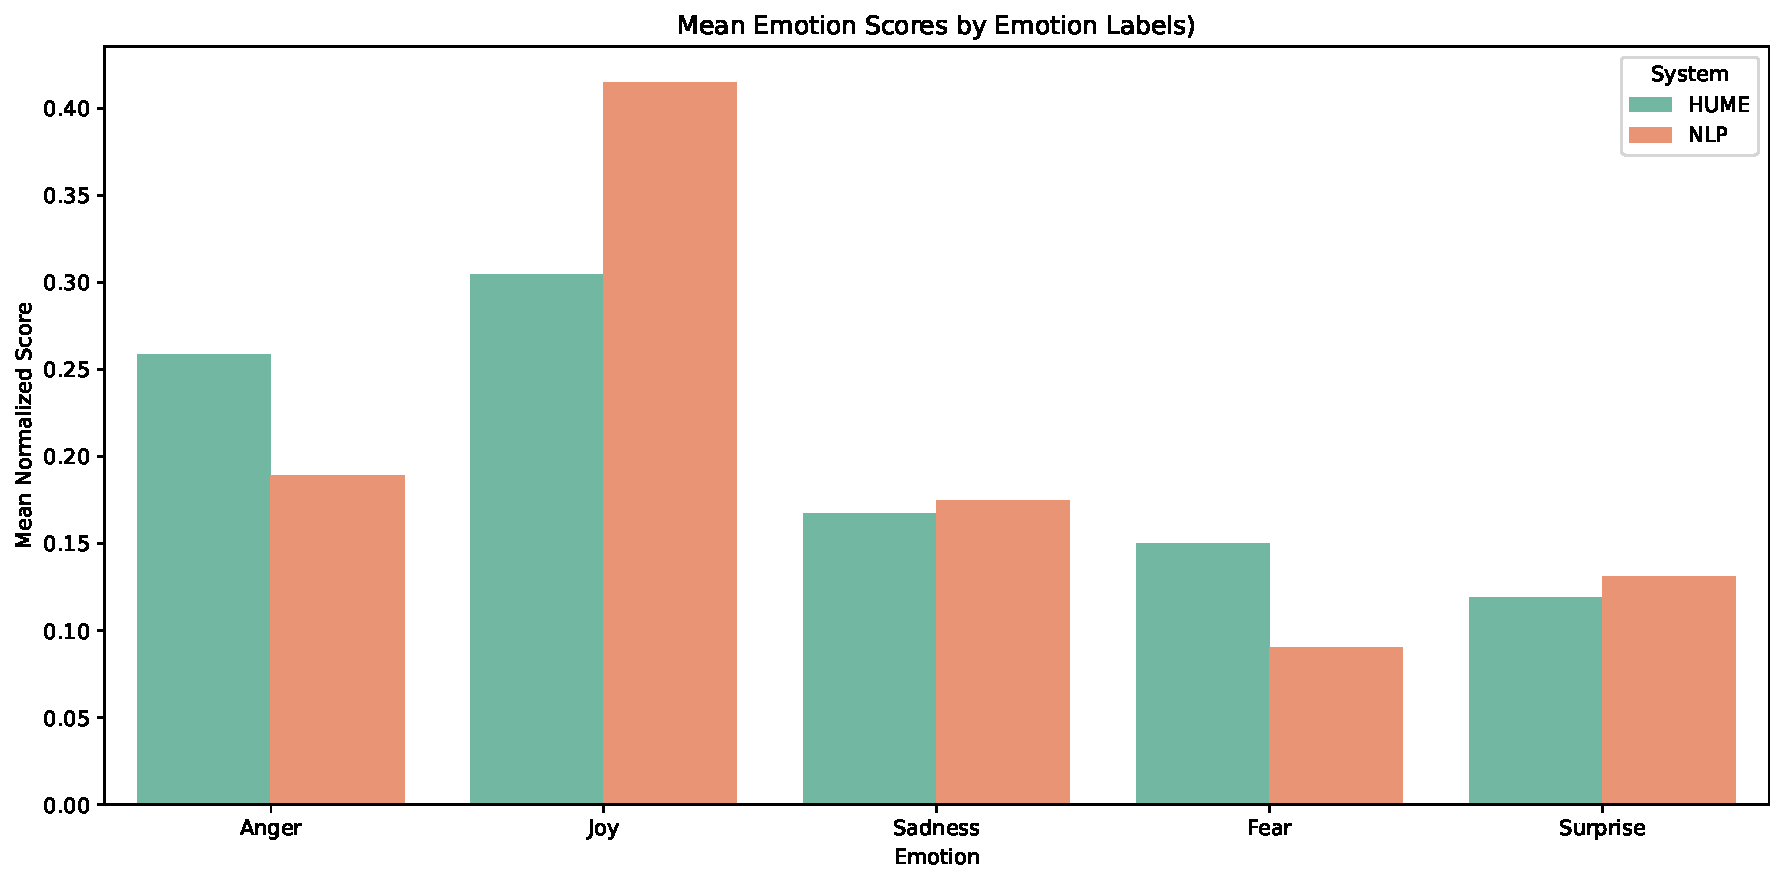
\includegraphics[width=0.7\textwidth]{png/results/rq2/sentiment_comparison_bar.pdf}
    \caption{Sentiment comparison bar for NLP and Hume.}
    \label{fig:sentiment-comp-rq2}
\end{figure}

\textbf{Positive Interviews}
Key Findings:
\begin{itemize}
    \item Anger was detected at significantly higher levels by Hume compared to NLP cloud, which rated Anger near zero. 
    This implies that Hume AI, that focuses on vocal tone, might pick up subtle vocal cues even when the participants are talking about positive memories. 
    NLP Cloud only analyzes textual content and does not interpret Anger when negative language is missing. 
    \item Joy is rated substantially high by NLP Cloud compared to both other emotions and Hume's probability. When participants discuss happy experiences, NLP 
    detects the emotion in high levels. Hume's lower detection for Joy might indicate that the expressed vocal features in the interview setting are less distinct,
    which leads to the underestimation. 
    \item Sadness and Fear are both rated higher than NLP, which gave these emotions minor scores. This aligns with that subtle negative undertones in speech, which could be due to reflective or 
    serious tones, are picked up by Hume in positive contexts. NLP misses these cues since nuances are not present in the transcribed content. 
    \item Surprise was detected at similar, low levels by both models. The emotion appears to be detected inconsistently, which may indicate that Surprise is difficult to capture, or rarely prominent in the recordings. 
\end{itemize}

\textbf{Negative Interviews}
Key Findings: 
\begin{itemize}
    \item Anger was somewhat higher rated by NLP than Hume. This indicate that NLP Cloud is sensitive to words expressed negatively, and may flag explicit language as anger. 
    Hume focuses on vocal tone, rated Anger slightly less, which can be due to vocal expressions being more controlled in an interview setting. 
    \item Joy was assigned higher by Hume than NLP in the negative interviews. Presumably due to the reason for the other emotions, where vocal patterns may be interpreted by Hume as positive even if its tied to a negative setting, 
    compared to NLP that devalued this emotion in comparison, probably because of negative transcriptions. 
    \item Sadness was detected at higher levels by NLP than Hume. 
    \item Fear and Surprise had similar detection results, with very small variation. This suggest that the emotions were expressed more consistently across both models, and the low levels that it might not be expressed prominent in the interviews overall. 
\end{itemize}

The text-based NLP Cloud is dependent on explicit emotional language, with highest rating for emotions that are clearly 
expressed in words, for example Joy in positive interviews, Anger and Sadness in negative interviews. 
The speech-based model Hume interprets vocal tones and may detect underlying emotional nuances, sometimes leading to unexpected results such 
as Joy in negative scenarios, Anger in positive scenarios. 

%%% T TESTS 
\subsubsection{Statistical Analysis}

Table \ref{tab:t-test-pos} demonstrates t-tests and Cohen's d for positive oriented interviews, where all emotions except for surprise shows significant differences 
with certainly large effect sizes. NLP have the aspects of overestimating Joy compared to Hume, where Hume in contrast tends to overestimate Anger in positive contexts. 
Hume rates Sadness and Fear more prominent than NLP, and Surprise remain inconsistent as previous results with no significant difference. 
The AI systems diverge significantly in positive interviews across almost all emotions, suggesting that text-based analysis can misinterpret 
emotional subtle cues, leading to inflating Joy. Hume may interpret vocal expressions in positive contexts as negative, probably due to the nature of the recordings, 
in agreement with previous results. 

 \begin{table}[!h]
    \centering
    \begin{tabular}{lllll}
    \multicolumn{5}{c}{\cellcolor[HTML]{C0C0C0}Positive Oriented Interviews}                                                                                                                                    \\
    \multicolumn{1}{c|}{\textbf{Emotion}} & \multicolumn{1}{c}{\textbf{t-statistic}} & \multicolumn{1}{c}{\textbf{p-value}} & \multicolumn{1}{c}{\textbf{Significant}} & \multicolumn{1}{c}{\textbf{Cohen's d}} \\ \hline
    \multicolumn{1}{l|}{Anger}            & 10,903                                   & 0                                    & Yes                                      & 2,815                                  \\
    \multicolumn{1}{l|}{Joy}              & -11,665                                  & 0                                    & Yes                                      & -3,012                                 \\
    \multicolumn{1}{l|}{Sadness}          & 6,177                                    & 0                                    & Yes                                      & 1,595                                  \\
    \multicolumn{1}{l|}{Fear}             & 5,125                                    & 0,0002                               & Yes                                      & 1,323                                  \\
    \multicolumn{1}{l|}{Surprise}         & -1,723                                   & 0,1069                               & No                                       & -0,445                                
    \end{tabular}
    \caption{t-statistics, p-value with significance, and Cohen's d for positive interviews.}
    \label{tab:t-test-pos}
\end{table}

Table \ref{tab:t-test-neg} presents conducted t-tests and Cohen's d in negative interviews, with significant differences for Joy, where Hume rates it significantly higher than NLP. 
In contrast, NLP has clear higher scoring for Sadness with large effects. 
Anger has a moderate difference, even if it is not statistically significant. No notable differences are detected for either Fear or Surprise. 
This implies that the AI systems strongly disagrees on Joy and Sadness detection in the negative contexts of the dataset. 

\begin{table}[!h]
    \centering
    \begin{tabular}{lllll}
    \multicolumn{5}{c}{\cellcolor[HTML]{C0C0C0}Negative Oriented Interviews}                                                                                                                                    \\
    \multicolumn{1}{c|}{\textbf{Emotion}} & \multicolumn{1}{c}{\textbf{t-statistic}} & \multicolumn{1}{c}{\textbf{p-value}} & \multicolumn{1}{c}{\textbf{Significant}} & \multicolumn{1}{c}{\textbf{Cohen's d}} \\ \hline
    \multicolumn{1}{l|}{Anger}            & -1,702                                   & 0,108                                & No                                       & -0,413                                 \\
    \multicolumn{1}{l|}{Joy}              & 3,72                                     & 0,0019                               & Yes                                      & 0,902                                  \\
    \multicolumn{1}{l|}{Sadness}          & -3,796                                   & 0,0016                               & Yes                                      & -0,921                                 \\
    \multicolumn{1}{l|}{Fear}             & 0,536                                    & 0,5993                               & No                                       & 0,13                                   \\
    \multicolumn{1}{l|}{Surprise}         & 1,311                                    & 0,2084                               & No                                       & 0,318                                 
    \end{tabular}
    \caption{t-statistics, p-value with significance, and Cohen's d for negative interviews}
    \label{tab:t-test-neg}
\end{table}

The emotional context impacts how the AI models detects emotions. Both systems presented larger differences in positive contexts, where vocal subtle cues and explicit language 
has different impact. 
NLP Cloud highly detects explicit emotions in text, especially Joy Anger and Sadness, but does not interpret subtle emotions such as Fear or Sadness in a positive context, since these emotions only might be expressed in nuanced vocal cues.
Hume AI captures these vocal nuances, resulting in detecting unexpected emotional states, such as Anger in positive interviews and Joy in negative ones. 
Which is affected by how something is said, where the tone can be opposing to the actual context. The speech-based model 
might overestimate negative emotions in reflective settings by this reason. 

Positive oriented interviews presents a wider divergence between the systems, which is confirmed by the large effect sizes. 
The negative interviews had more consistent detection, except for Joy and Sadness that had significant differences. 
For surprise, detection challenges or lack of expression of that emotion in the interviews might impacting the results of no significant difference for both sentiment contexts. 

In conclusion, the sentiment-based analysis shows that AI emotion detection in sensitive to both context and the modality. 
Text-based analysis has higher performance in identifying the explicit stated emotions, while speech-based 
analysis reveals deeper and probably more subtle emotional cues. 
These results suggests that none of the systems provides a universally accurate interpretation across all emotions,
which indicates that text and speech-based emotion detection has limitations. 


\subsubsection{Case Example}
single clip comparison 

breifly illustrate how speech vs text differ in practice 



%%%%%% RQ3%%%%%%%%%%%%%%%

\section{Data Analysis for RQ3: AI and self-assessed emotion labels}

The third research question explores how AI-generated emotion labels - from both speech-based (Hume AI) and text-based (NLP Cloud) 
analyses - aligns with self-assessed emotions. It is of importance to understand how these AI systems reflect humans perception of 
their own emotions and explore how the systems align with the participants own emotional viewpoint.  
\subsection{Descriptive Overview}

For an initial overview, Table~\ref{tab_summery-rq3} summerizes the average emotion scores across all 32 interview recordings 
for each emotion category (Anger, Joy, Sadness, Fear, Surprise). The table presents mean values and standard deviation for self-resported scores 
aside both AI-systems.

\begin{table}[!h]
    \centering
    \begin{tabular}{c|llllll}
    \textbf{Emotion}  & \multicolumn{1}{c}{\textbf{Self Mean}} & \multicolumn{1}{c}{\textbf{Hume Mean}} & \multicolumn{1}{c}{\textbf{NLP Mean}} & \multicolumn{1}{c}{\textbf{Self Std}} & \multicolumn{1}{c}{\textbf{Hume Std}} & \multicolumn{1}{c}{\textbf{NLP Std}} \\ \hline
    \textbf{Anger}    & 0,21                                   & 0,26                                   & 0,2                                   & 0,124                                 & 0,072                                 & 0,223                                \\
    \textbf{Joy}      & 0,312                                  & 0,302                                  & 0,396                                 & 0,2                                   & 0,117                                 & 0,351                                \\
    \textbf{Sadness}  & 0,19                                   & 0,167                                  & 0,181                                 & 0,105                                 & 0,065                                 & 0,138                                \\
    \textbf{Fear}     & 0,136                                  & 0,15                                   & 0,093                                 & 0,061                                 & 0,045                                 & 0,092                                \\
    \textbf{Surprise} & 0,149                                  & 0,118                                  & 0,129                                 & 0,082                                 & 0,022                                 & 0,089                               
    \end{tabular}
    \caption{Mean and standard deviation for Hume, NLP, and Self-labels for the full dataset.}
    \label{tab:summery-rq3}
\end{table}

As shown in the table, Joy consistently has the highest average scores across all sources, in certain for NLP Cloud,
which has a notable higher mean value (0.396) compared to self-reports (0.312) and Hume (0.302). 
In contrast, emotions as Fear and Surprise have a tendency for lower average scores, where both AI-systems generally assigns these 
emotion labels slightly lower for these emotions compared to the participants own scoring. 

To visualize these differences, Figure~\ref{fig:comp-bar-rq3-all} illustates a bar chart that compares the average emotion scores defined by 
participants self-assessment, Hume AI and NLP Cloud. 

\begin{figure}[!h]
    \centering
    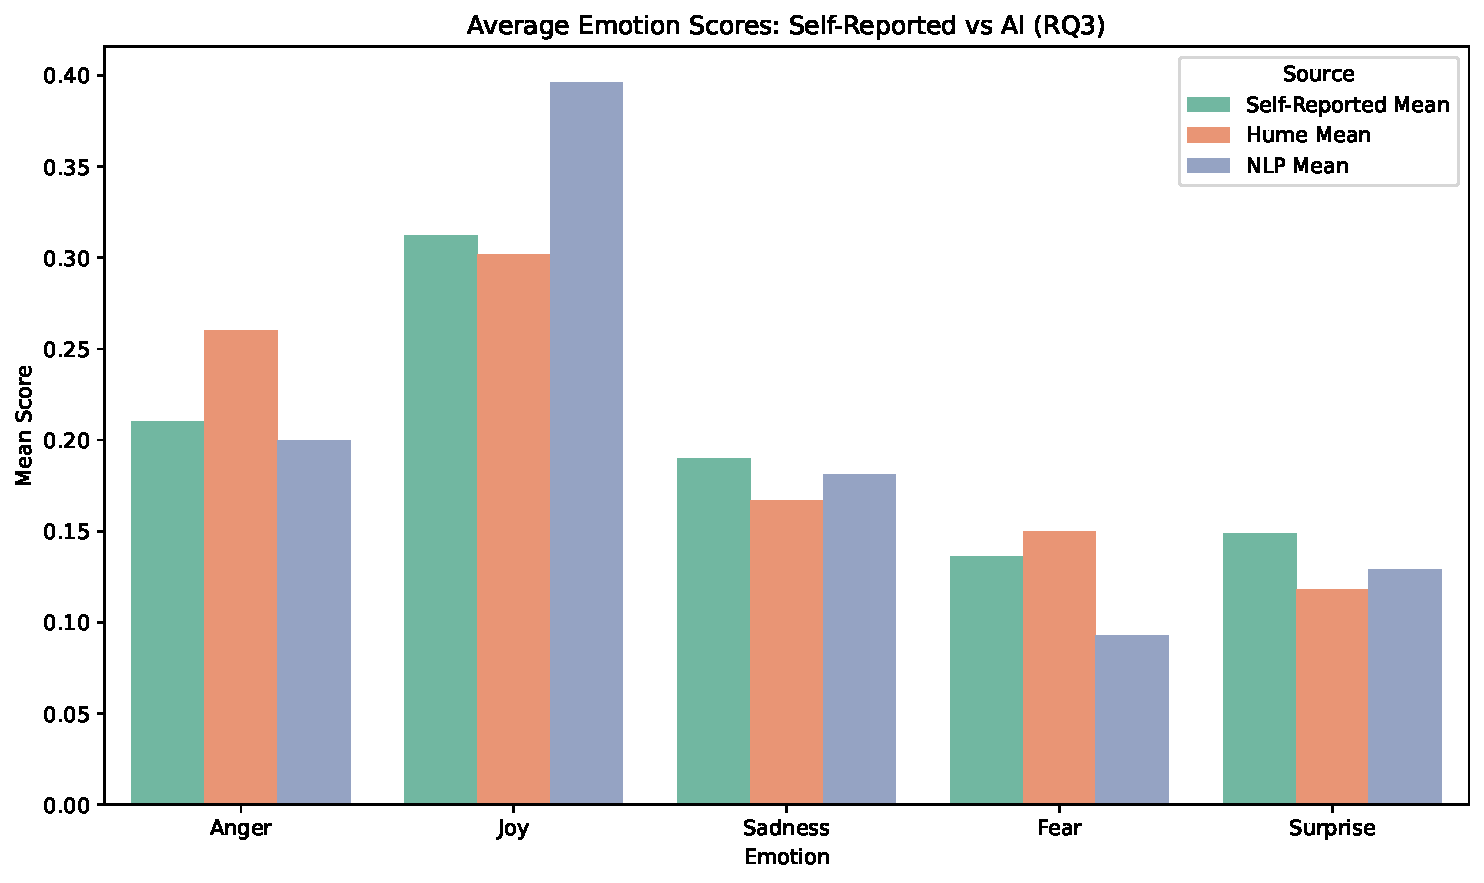
\includegraphics[width=0.7\textwidth]{png/results/rq3/rq3_emotion_comparison.pdf}¨
    \caption{Comparison of emotional labels for Hume, NLP, and self-assessed.}
    \label{fig:comp-bar-rq3-all}
\end{figure}

Key patterns from bar chart \ref{fig:comp-bar-rq3-all}:
\begin{itemize}
    \item NLP Cloud tends to overestimate Joy compared to both self-reported and Hume's emotion labeling. 
    \item For Anger, self and NLP-labeling are highly congurent, while Hume assigns higher average scores.
    \item Regarding Sadness and Surprise, the AI systems tends to report moderately lower scores than the participants, particularly for Surprise. 
    \item Sadness, Fear, and Surprise are consistently rated lower across all sources, especially Fear and Surprise, where Hume tends to rate Fear more frequent than the other, and self-labels has a higher surprise score than the other sources.
\end{itemize}
This comparison suggests that even if general alignment in emotional ranking occur, where Joy is most prominent across all sources, both AI systems 
demonstrate differences compared to human self-perception. Particularly NLP Cloud that appears to be more prone to rating Joy, while Hume provides more moderate scores, although all sources tends gravitate towards high scores for emotions Anger and Joy. 

These insights compose the framework for further statistical analysis, where correlation analysis and significance tests will 
be used to evaluate the strenghts and consistency of these patterns. 

\subsection{Correlation and Visual Analysis}
- pearson correlation p value 

+ scatter plots 

- interpret these 
- which emotion show strongest corerlation between ai and human perception 
note weak or non-significant correlations 
discuss if speech based or text based aligns best 

To evaluate the alignment between AI-generated emotion scores and participants self-reported emotions, 
Pearson correlation analyses were conducted across the five emotion categories for both speech-based (Hume AI) and text-based (NLP Cloud) compared to self-reporting.
With these measurements the relationship's strength and direction and the statistical significance can be reviewed. 

\subsubsection{Hume AI vs Self-Reported Emotions}
The correlation results for Hume AI is demonstrated in Table~\ref{tab:corr-hume-self}, and indicate generally weak correlations across the majority of emotions. 
Anger is the only emotion showing a statistic significant correlation (r = 0.359, p = 0.043), which indicates a moderate alignment between Hume AI's speech based emotion 
detection and participants own perception for this emotion. Other emotions, such as Fear (r = 0.007, p = 0.969), presents no relevant correlation. 

It is of importance to note that Hume AI analyzes vocal expression patterns, such as vocal bursts and porosody, rather than the semantic content of the recorded speech. 
Considering the interview setting that the recordings which complies the data collection, where participants recalled past emotional experiences in a controlled environment, 
the extent to which emotions were expressed vocally may vary, that potentially incluence the correlation results. 

%%% Correlation hume self 

\begin{table}[!h]
    \centering
    \begin{tabular}{cll}
    \multicolumn{3}{c}{\cellcolor[HTML]{C0C0C0}Hume vs Self-Assessed}                                                        \\
    \multicolumn{1}{c|}{\textbf{emotion}}  & \multicolumn{1}{c}{\textbf{pearson\_r}} & \multicolumn{1}{c}{\textbf{p\_value}} \\ \hline
    \multicolumn{1}{c|}{\textbf{anger}}    & 0,359                                   & 0,043                                 \\
    \multicolumn{1}{c|}{\textbf{joy}}      & 0,334                                   & 0,062                                 \\
    \multicolumn{1}{c|}{\textbf{sadness}}  & 0,050                                   & 0,784                                 \\
    \multicolumn{1}{c|}{\textbf{fear}}     & -0,007                                  & 0,969                                 \\
    \multicolumn{1}{c|}{\textbf{surprise}} & 0,088                                   & 0,631                                
    \end{tabular}
    \caption{Correlation and p-value for Hume AI and self reporting.}
    \label{tab:corr-hume-self}
\end{table}

%%% Self vs NLP 
\subsubsection{NLP Cloud vs Self-Reported Emotions}
\label{sec:nlp-self}
NLP Cloud demonstrated strong and statistically significant correlations for four of five emotions, see 
Table~\ref{tab:corr-nlp-self}. 

\begin{table}[!h]
    \centering
    \begin{tabular}{cll}
    \multicolumn{3}{c}{\cellcolor[HTML]{C0C0C0}NLP vs Self-Assessed}                                                         \\
    \multicolumn{1}{c|}{\textbf{emotion}}  & \multicolumn{1}{c}{\textbf{pearson\_r}} & \multicolumn{1}{c}{\textbf{p\_value}} \\ \hline
    \multicolumn{1}{c|}{\textbf{anger}}    & 0,739                                   & 0,00000                               \\
    \multicolumn{1}{c|}{\textbf{joy}}      & 0,863                                   & 0,00000                               \\
    \multicolumn{1}{c|}{\textbf{sadness}}  & 0,710                                   & 0,00001                               \\
    \multicolumn{1}{c|}{\textbf{fear}}     & 0,669                                   & 0,00003                               \\
    \multicolumn{1}{c|}{\textbf{surprise}} & 0,092                                   & 0,61569                              
    \end{tabular}
    \caption{Correlation and p-value for NLP Cloud and self reporting.}
    \label{tab:corr-nlp-self}
\end{table}

Key Findings: 
\begin{itemize}
    \item Joy showed a very strong correlation (r = 0.863, p < 0.0001). 
    \item Anger and Sadness had very high correlation values (Anger: r = 0.793, Sadness: 0.710), with extremely low p-values for both emotions. 
    \item Fear had a moderately strong correlation (r = 0.67, p = 0.00003), with considerably statistical significance. 
    \item Surprise had no statistical significance and weak correlation (r = 0.092, p = 0.616). 
\end{itemize}
Text-based emotion detection with NLP shows a explicit correlation with self-reported emotions for four out of five emotions. The emotion scoring certainly similar for Anger, Joy, Sadness and Fear. 
Surprise was the only emotion that did not show a significant correlation for NLP and self-perceived emotion labels. Surprise is the one emotion both AI-systems concurrently failed to show a significant correlation, 
which suggests that the models have difficulties in detect these emotions accurately. However, this inconsistency may not reflect limitations of the 
AI-systems. During data collection, several participants expressed challenges in assessing their level of Surprise and had difficulties understanding how to rate that emotion, 
this indicates both potential variablity and misunderstanding in self-reported scores for Surprise. 
Therefore, the low correlation for Surprise could be associated to unreliable self-assessments, rather than a underlying weakness in AI-based detection. 


\subsubsection{Visual Correlation}
To illustrate the correlations between AI-labels and self-reported emotions, 
%% ANGER
\begin{figure}[!h]
    \centering
    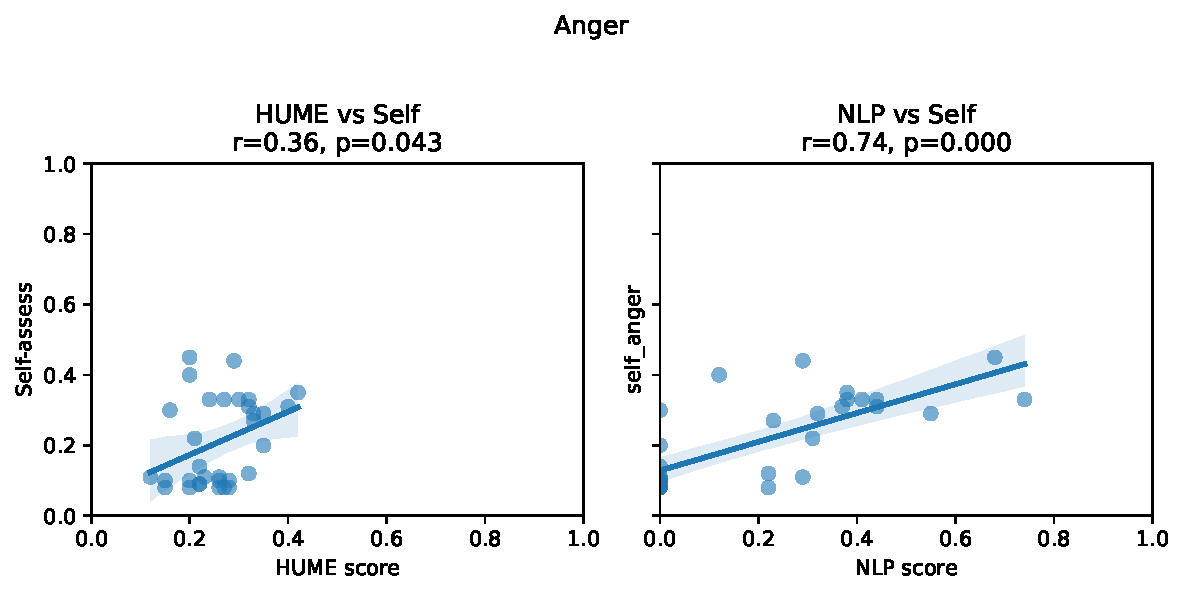
\includegraphics[width=0.7\textwidth]{png/results/rq3/scatter_anger_vs_self.pdf}
    \caption{Scatter plot, Hume, NLP vs. Self for Anger.}
    \label{fig:scatter-anger-rq3}
\end{figure}

%% JOY
\begin{figure}[!h]
    \centering
    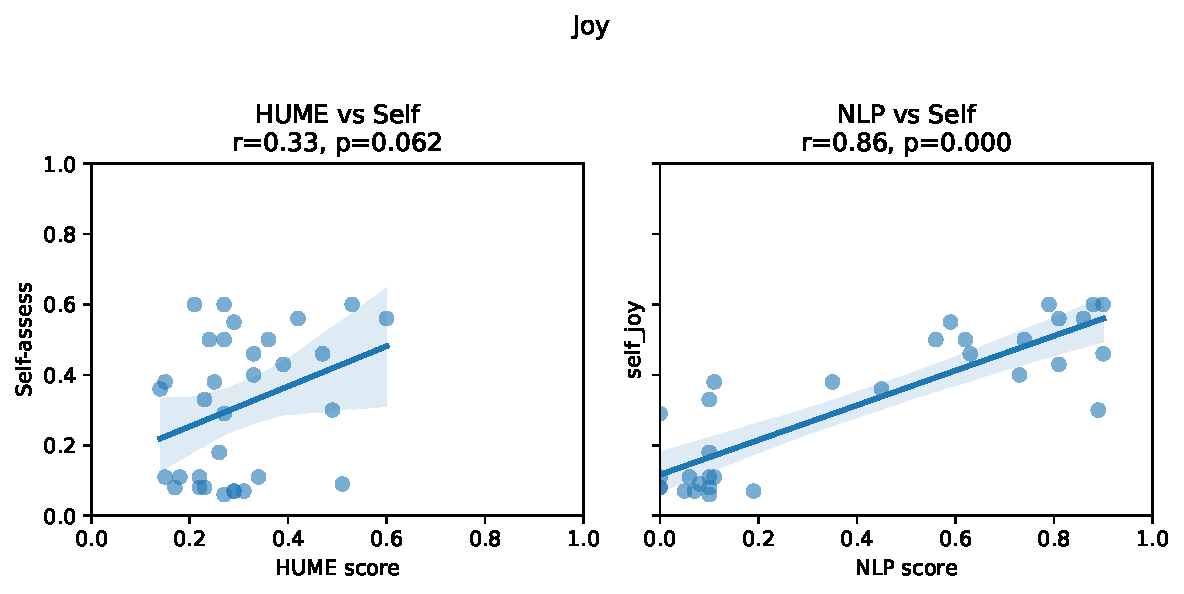
\includegraphics[width=0.7\textwidth]{png/results/rq3/scatter_joy_vs_self.pdf}
    \caption{Scatter plot, Hume, NLP vs. Self for Joy.}
    \label{fig:scatter-joy-rq3}
\end{figure}

%% SURPRISE 
\begin{figure}[!h]
    \centering
    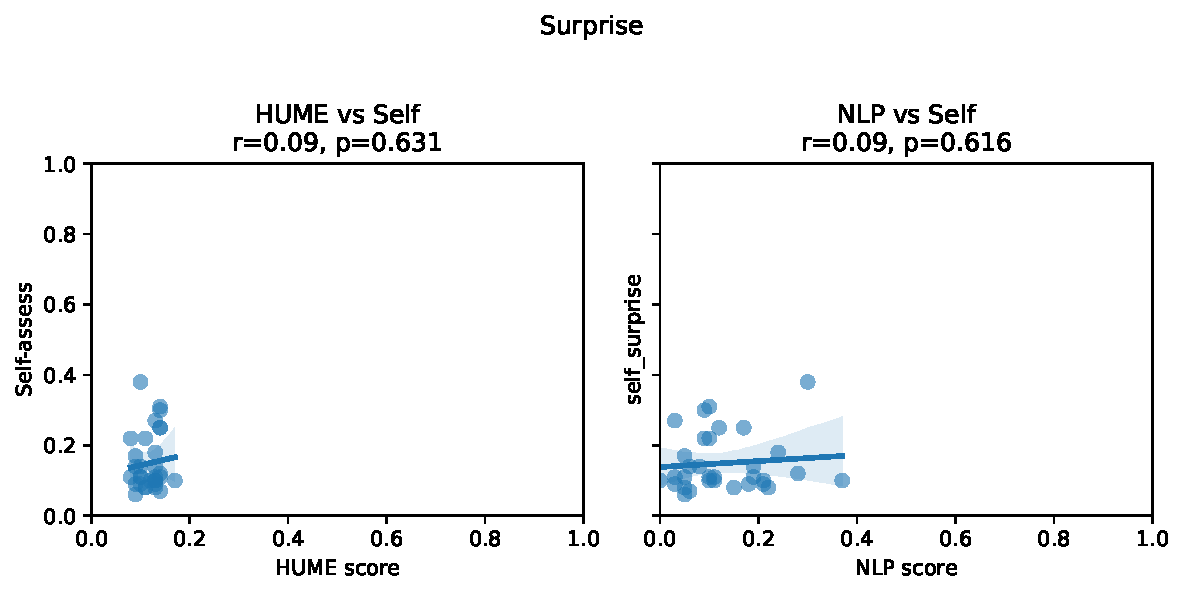
\includegraphics[width=0.7\textwidth]{png/results/rq3/scatter_surprise_vs_self.pdf}
    \caption{Scatter plot, Hume, NLP vs. Self for Surprise.}
    \label{fig:scatter-surprise-rq3}
\end{figure}

\newpage 
\subsection{Statistical Analysis and Effect Sizes}

To explore if AI-generated emotion scores has a significant difference from self-reported emotions, paired t-tests were conducted for both Hume AI and NLP Cloud across each emotion. 
To evaluate the effect size of these differences, Cohen's d were calculated. These results are presented in Table~\ref{tab:t-test-rq3}.
\begin{table}[!h]
    \centering
    \begin{tabular}{l|lllll}
    \textbf{System} & \textbf{Emotion} & \textbf{t-statistic} & \textbf{p-value} & \textbf{Significant} & \textbf{Cohen's d} \\ \hline
    HUME            & Anger            & 2,399                & 0,023            & Yes                  & 0,424              \\
    NLP             & Anger            & -0,373               & 0,711            & No                   & -0,066             \\
    HUME            & Joy              & -0,271               & 0,788            & No                   & -0,048             \\
    NLP             & Joy              & 2,331                & 0,026            & Yes                  & 0,412              \\
    HUME            & Sadness          & -1,069               & 0,293            & No                   & -0,189             \\
    NLP             & Sadness          & -0,525               & 0,603            & No                   & -0,093             \\
    HUME            & Fear             & 1,052                & 0,301            & No                   & 0,186              \\
    NLP             & Fear             & -3,496               & 0,001            & Yes                  & -0,618             \\
    HUME            & Surprise         & -2,109               & 0,043            & Yes                  & -0,373             \\
    NLP             & Surprise         & -1,011               & 0,320            & No                   & -0,179            
    \end{tabular}
    \caption{T-statistics, p-value and Cohen's d for AI-models and self-assessed emotions.}
    \label{tab:t-test-rq3}
\end{table}

\textbf{Key Findings:}
\begin{itemize}
    \item Hume AI: 
    \begin{itemize}
        \item Anger (p = 0.023) and Surprise (p = 0.043) showed significant differences. 
        \item Both Anger and Surprise showed small to moderate effect sizes (Cohen's d > 0.4), which suggests that Hume AI tends to overestimate Anger and underestimate Surprise compared to self-reported emotion scores. However, as declared in NLP vs. Self-Reported emotions~\ref{sec:nlp-self}, particpants stated confusion regarding assessing Surprise.
        \item For the other emotions, Joy, Sadness, and Fear, no significant differences were found, suggesting closer average alignment for these emotions.
    \end{itemize}
    \item NLP Cloud: 
    \begin{itemize}
        \item Joy (p = 0.026) and Fear (p = 0.001) presented significant differences. 
        \item Fear had a particularly evident difference, (Cohen's d = -0.618) states a medium-to-large effect size, indicating that NLP Cloud underestimated Fear compared to self-reported emotion scores. 
        \item Joy had a small-to-moderate effect size (Cohen's d = 0.412), suggesting that NLP overestimated Joy compared to the participants own perception. 
        \item Anger, Sadness, and Surprise showed no significant difference. 
    \end{itemize}
\end{itemize}
\textbf{General Analysis:}

Both AI systems demonstrates some alignment with self-reported emotions, the results indicate certain biases. Self reported emotion scores appears to be more prone to diverge from Hume AI's detection of Anger and Surprise. 
Regarding NLP Cloud, the emotion scores are distinct from self-assessed emotions for Fear and Joy, where Fear is most prominent. This could indicate either challenges in text-based detection of these subtle, negative emotions, 
or challenges for the participants to assess these emotions. 

Even where statistical significance is found, the effect size implies that most differences are small to moderate, which 
suggests that even if deviations exists, they are not disturbingly large. It is no consistent significant difference for the AI-systems across all emotions, proposing that AI performance may vary depending on emotional category and the method (speech vs text, and different AI-models).
However, it is important to emphasize that these results may not fully reflect the performance or accuracy of the
AI models, as the analysis are based on a small dataset with semi-structured interviews. Furthermore, disparity and miscalculations may arise from challenges participants experienced in assessing their own emotions after each interview. 

\medskip
Overall, these findings suggest that AI systems can approximate human emotional self-assessment with partial alignment, some differences still appear depending on emotion and detection method. 
Hume AI had more diverse scores for Anger and Surprise, while NLP Cloud was more distinct for Fear and Joy. The differences may reflect some challenges in AI detection or difficulties for the participants to assess their emotions accurately. 

Even if some differences were significant statistically, the effect sizes indicate that they are generally small to moderate. There is no consistent pattern across all emotions which indicates that the AI performance vary by emotion category and analysis method (speech vs text).
\medskip

Considering the small dataset, the subjective nature of self-assessment, and the recording circumstances of the interview setting, these findings should be interpreted 
carefully and should be seen as exploratory and not conclusive. 


%%%%% SENTIMENT rRQ3 %%%%%% 
\subsection{Sentiment-Based Analysis}
To explore how AI-generated emotion labels and self-reported emotions align, a sentiment-based analysis have been conducted through seperation of negative and positive interviews. 
Each participant reported scores (1-6 scale, normalized to 0-1) for all five emotions after each interview-scenario, without considering wheather the interview was directed positevly or negatively. 

Since the majority of emotions are perceived negative (Anger, Sadness, Fear), the negatively directed interviews have more spread results than the positive ones. 
The interviews were intentionally structured to provoke either positive or negative emotions using guided questions based on autobiographical recall techniques. 
The setup allowed for a clear distinction between these emotional contexts and enabled analyzation on potential differences in emotion recognition. 
However, it is important to state that these categorization does not represent an ground truth, since the participants emotional states may not fully align with the intended positive or negative orientation throughout the interviews. 

As expected, the participants generally rated Joy higher for positive interviews, as well as negative directed interviews had more prominent scores Anger, Sadness, and Fear. 
Since all emotions were rated in both scenarios, variations for the sentiment categories provides insights in how AI systems provide emotional tones, in the context of our dataset. 

Figure~\ref{fig:sentiment-bar-rq3} illustrate the average emotion scores for positive and negative interviews for Hume AI, NLP Cloud, and self-assessment. 
When interpreting these results, it is important to note that participants actual emotional expressions, particularly vocally, may not be fully aligned with the intention to evoke distinct emotional tones, due to the reflective and conversational nature of the setting.
\begin{figure}[!h]
    \centering 
    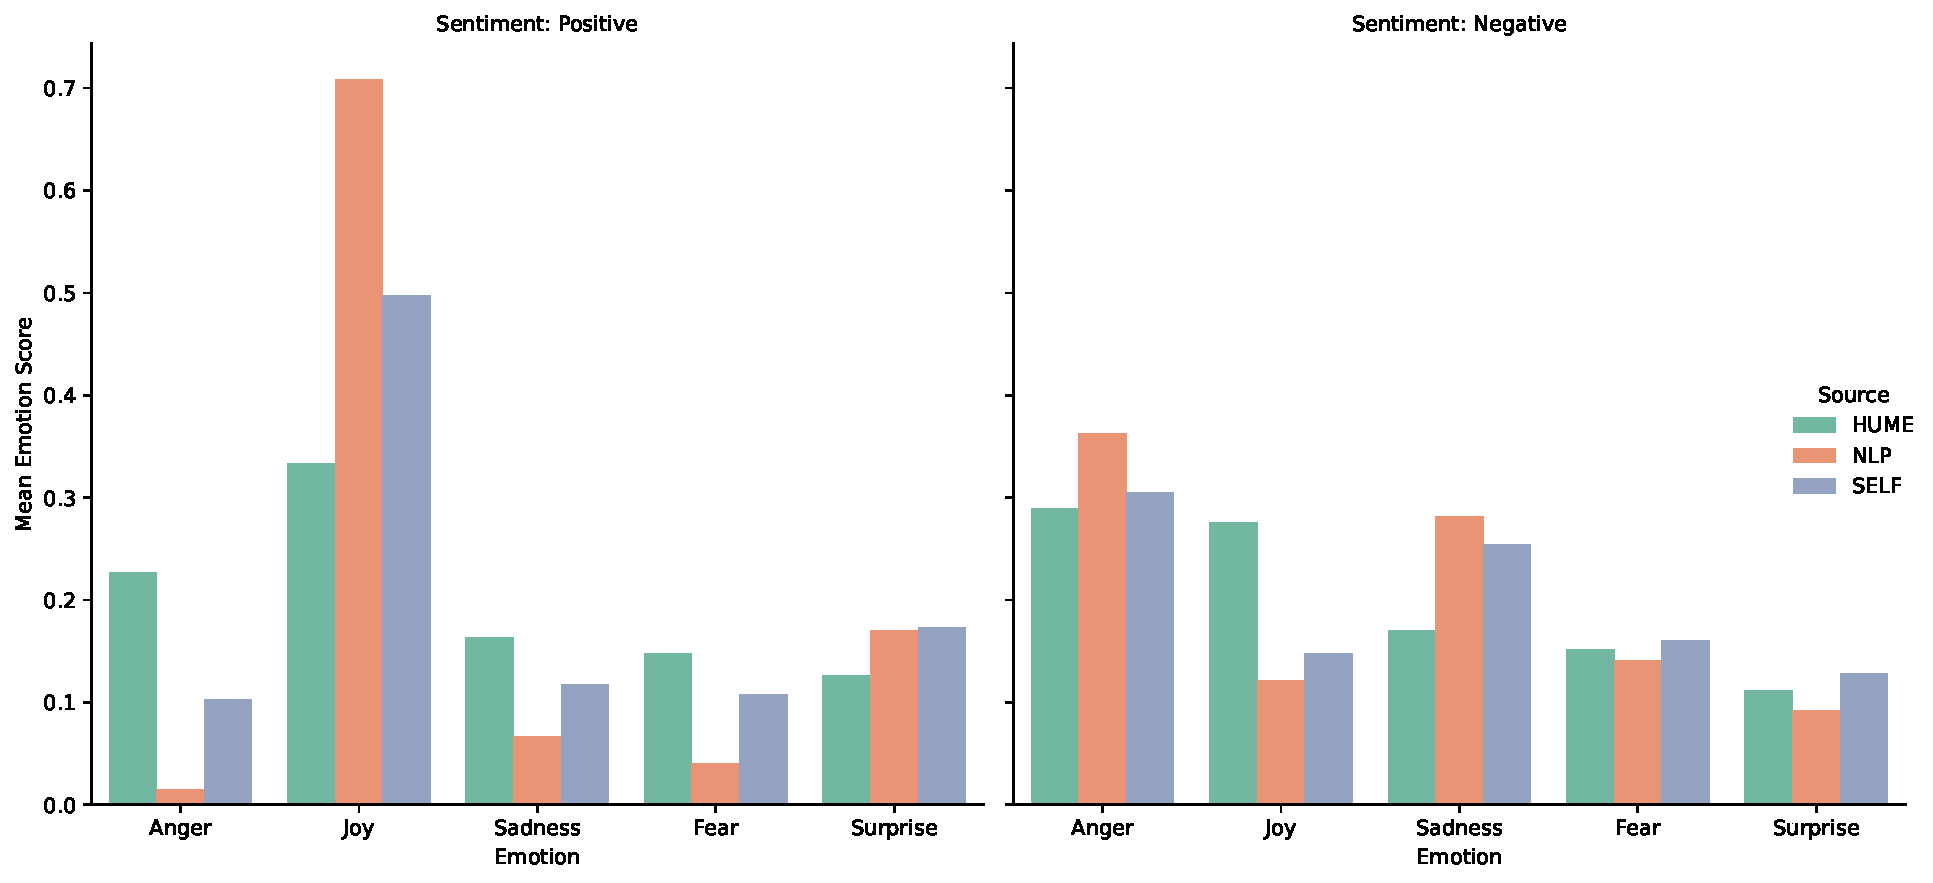
\includegraphics[width=0.7\textwidth]{png/results/rq3/rq3_sentiment_grouped_bar.pdf}
    \caption{Emotion scores for all sources grouped by sentiment.}
    \label{fig:sentiment-bar-rq3}
\end{figure}


\textbf{Positive Interviews}

In positive interviews, NLP Cloud consistently rated Joy higher, in agreement with previous results. The difference from self-reported joy is similar, although NLP tends to rate it moderately higher. 
This reflect the strength of text-based detection for explicit positive sentiment when analyzed as a transcription. 

%% MOVE to RQ2  WRITE SHORTER FOR RQ3 
Both AI systems detected negative emotions minimally, but it is notable that Hume AI detected Anger, Sadness, and Fear more prevalent than NLP and self-reports. 
This suggest that subtle vocal expressions, such as tone or pitch, may have been interpreted by Hume as indicators of negative emotions, even when the participants talked about positive memories. 
This is aligned with the understanding that individuals may not express positive emotions vocally as distinct when talking in a reflective interview setting. 

For surprise, both self-reports and NLP had similar rating, while Hume had moderately lower detection, which is consistent with previous observations about the AI systems difficulty in detecting this emotion. 

\medskip
\textbf{Negative Interviews}

In negative oriented interviews, Hume and self-reports showed highly correlated anger scores, while NLP rated this slightly higher - likely due to that the transcripts consists of explicit negative language. 
In contrast, Hume rated Joy unexpectedly high compared to NLP and self-reports. This might indicate that some vocal patterns were misinterpreted by the speech-based model as positive emotional cues. 

For sadness, NLP had higher scores than Hume, and are more aligned with self-reported values. All three sources showed similar scores for fear and surprise, suggesting a more consistent detection for these three emotions in context of negative interviews.

\medskip
\textbf{Conclusion}


